\svnid{$Id$}
\chapter{Nitrite Reduction in \Nm{}}
\label{chap:nitritereduction}

%In the case of this dataset, nitrite reduction has been modelled very well, but nitric oxide (and to a small extent, oxygen) has not been [Caveat, this may change when the cluster does eventually spit out the complete trajectory. This then could be moved into the discussion about why priors are important]. Not shown in Figure \ref{fig:no2sim} is the concentration of nitric oxide as nitrite is reduced. Unfortunately the parameter set used to generate the solved output assigned a very low value to the concentration of NorB (even though this should have been being expressed), thus the nitric oxide produced by reduction of nitrite does not itself get reduced, and towards the end of the dataset would be lethal to the culture. In this case, a different prior distribution should have been used for NorB concentration, as it was known beforehand that NorB concentration would be non-zero. This is an example of why the prior distributions are important.

\section{Microerobic Nitrite Reduction}
% \subsection{Introduction}
% \subsection{Results}
% \subsection{Discussion}
% \section{\texorpdfstring{Microaerobic Nitrite Reduction in \textit{norB$^\textrm{-}$} mutant}{Microaerobic Nitrite Reduction in norB- mutant}}
% \subsection{Introduction}
% \subsection{Results}
% \subsection{Discussion}
% \section{\texorpdfstring{Aerobic Nitrite Reduction in \textit{nsrR$^\textrm{-}$} mutant}{Aerobic Nitrite Reduction in nsrR- mutant}}
\subsection{Introduction}

The last datasets to be used in the iterative approach to parameter estimation was of cultures able to respire nitrite in addition to oxygen. In these cultures nitrite was added to a culture already respiring oxygen to observe both the rate of nitrite reduction, and the effect on oxygen respiration caused by the production of nitric oxide. These datasets were the most complex in terms of the information contained within them and the number of model components needed to solve them. In addition to the components being used to model nitric oxide reduction, the nitrite reduction pathway is also active. The portions of the ETC relating to nitrite reduction are shown graphically in Figure \ref{fig:no2_resp_chain}. However since \Nsm{} is incapable of growing anaerobically, in actual fact the entire pathway is required, using oxygen nitric oxide and nitrite reduction.
\begin{figure}[tbp]
  \centering
    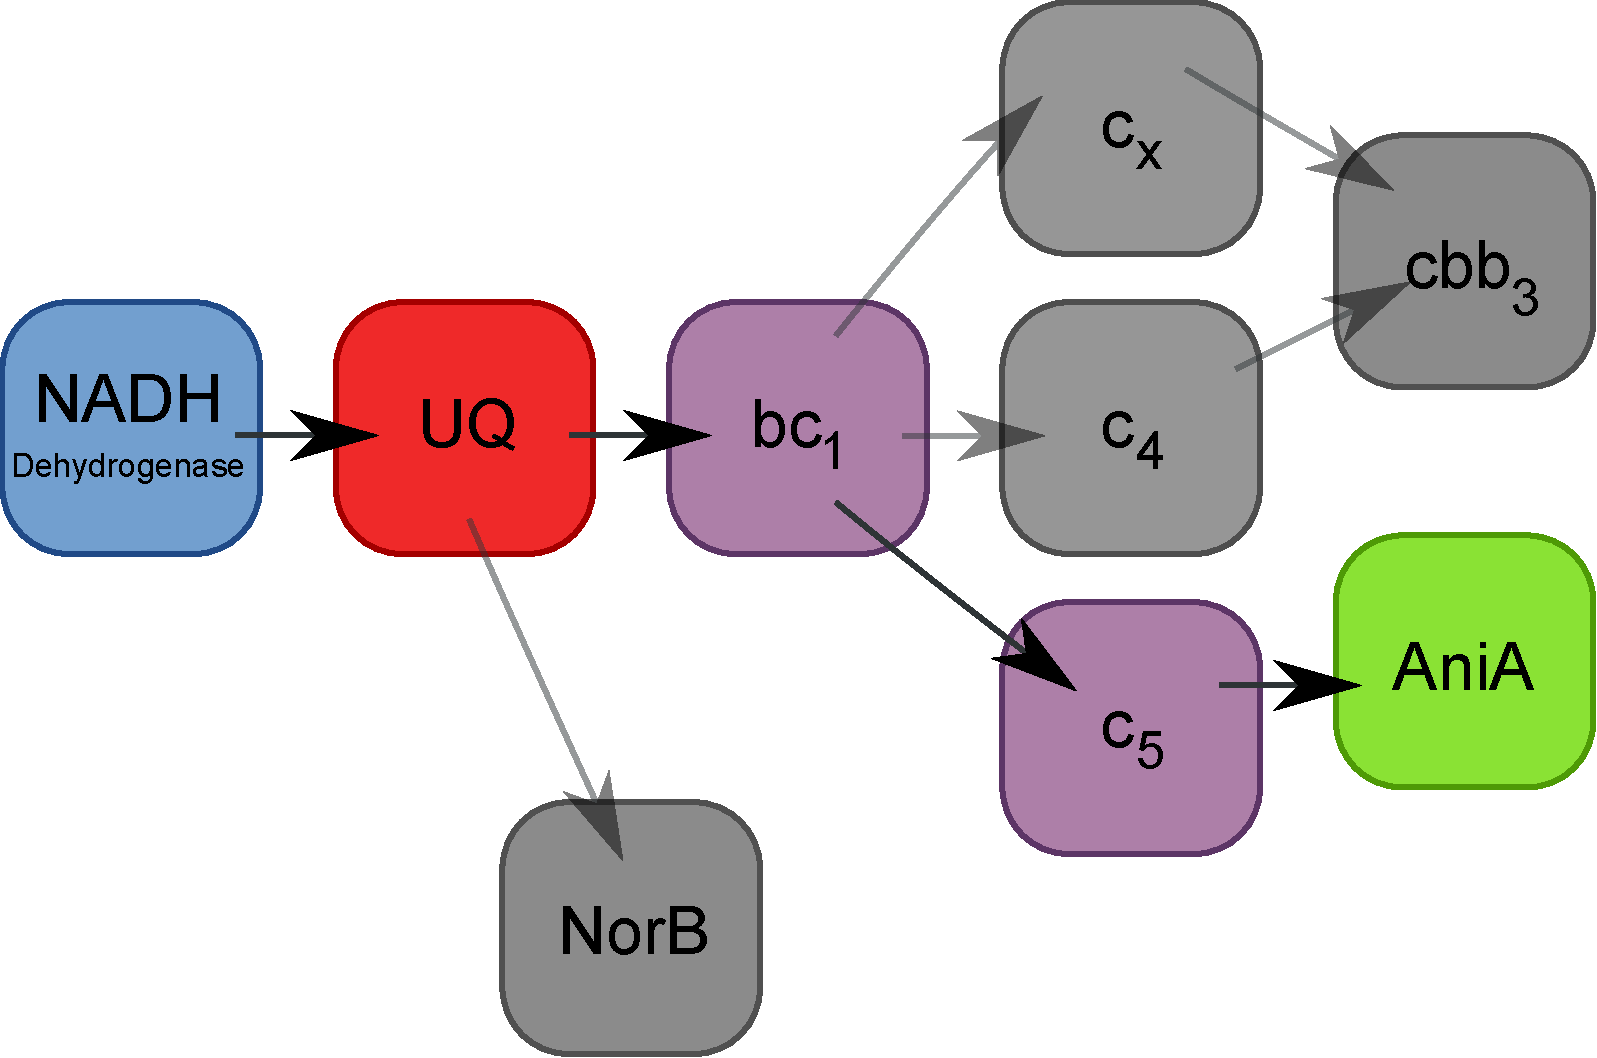
\includegraphics[width=14cm]{07-nitritereduction/data/no2_resp_chain.pdf}
    \caption[Nitrite reducing electron transport chain of \Nm{}]{{\bf Nitrite reducing electron transport chain of \Nm{}.} This shows the complete electron transport chain of \Nsm{} with the components irrelevant to nitrite reduction greyed out. In the mathematical model all of the purple elements (cytochromes) are amalgamated into one entity.
  \label{fig:no2_resp_chain}}
\end{figure}

\noindent The equations that describe this portion of the ETC are:
\begin{eqnarray*}
\frac{d[O_2]}{dt} & = & \beta(1-[O_2]/K_O) - k_{1}[C_a][O_2]\\
\frac{d[Q_a]}{dt} & = & g([Q] - [Q_a]) - l_3[Q_a]([B] - [B_a]) - f[Q_a]([X]-[X_a])\\
\frac{d[X_a]}{dt} & = & -k_3([C] - [C_a] - [C_X])[X_a]  - m_3([A] - [A_a])[X_a] + f[Q_a]([X]-[X_a])\\
\frac{d[C_a]}{dt} & = & k_3([C] - [C_a] - [C_X])[X_a] - k_{1}[C_a][O_2] - k_5[C_a][NO] + k_6[C_X]\\
\frac{d[NO]}{dt} & = & m_{1}[NO_2^-][A_a] - l_1[NO][B_a] - k_5[C_a][NO] + k_6 [C_X] - \gamma[NO]\\
\frac{d[NO_2^-]}{dt} & = & - m_{1}[NO_2^-][A_a]\\
\frac{d[C_X]}{dt} & = & k_5[C_a][NO] - k_6 [C_X]\\
\frac{d[A_a]}{dt} & = & m_3([A] - [A_a])[X_a]- m_{1}[NO_2^-][A_a]\\
\frac{d[B_a]}{dt} & = & l_3[Q_a]([B] - [B_a]) - l_1[NO][B_a]
\end{eqnarray*}

These equations describe the change in concentration of nitrite over time, which is the experimentally observed value (in addition to the afore modelled oxygen and nitric oxide). Also modelled is the reduction state of AniA. This represents the complete mathematical model not including any transcriptional parameters.

\subsection{Experimental Results}
Generating datasets for Nitrite reduction could be performed in with two different cultures; an aerobic NsrR deficient mutant, or microaerobic wild-type. Microaerobic cultures appeared to grow very poorly during the course of this work and in most cases did not survive the transition from being in the incubator to being moved to the electrode chamber. Therefore an $nsrR^-$ mutant was used instead of the wild-type. This mutant expresses AniA and NorB in a constitutive manner, removing the necessity for growing the cultures in microaerobic conditions. The cultures were grown in aerobic conditions until mid-log phase growth had been achieved. This corresponded to an $OD_{600}$ of $0.3-0.9$ and usually required an incubation period of roughly 3 hours. Once the required cell density had been obtained the culture was transferred to the electrode chamber, Sodium Nitrite was added to a concentration of 1 mM and the nitrite and oxygen concentrations recorded as the culture respired. Unfortunately nitric oxide concentrations could not be recorded as the NO electrode had failed and could not be replaced.

In addition to the datasets obtained from $nsrR^-$ mutant cultures, a further dataset was obtained from \citet{Rock2005} which showed oxygen and nitric oxide concentrations in a microaerobic wild-type culture where nitrite is added partway through aerobic respiration. The datasets generated and used for parametrisation of this portion of the model are shown in Figures \ref{fig:nitriteds1} \& \ref{fig:nitriteds2}.

The dataset in Figure \ref{fig:nitriteds1} shows an $nsrR^-$ mutant which has had 1mM nitrite added at $t=0s$. Nitrite reduction proceeds linearly and at quite a high rate. Oxygen starts linearly but then slows down presumably as nitric oxide is produced and inhibits \cbbthree{}. It is also possible that given the high rate of nitrite reduction large quantities of nitric oxide are being produced which will react directly with oxygen as described in Chapter \ref{chap:noreduction} affecting the rate of observed oxygen reduction.

The dataset in Figure \ref{fig:nitriteds2} shows a wild-type culture grown in denitrifying conditions, so that it is expressing both AniA and NorB. Nitrite is added at time $t\approx200s$ to a concentration of $\approx 1$ mM (Moir, private communication). Upon nitrite addition a small decrease in oxygen respiration rate is observed, and a large increase in nitric oxide occurs as nitrite is reduced. Nitric oxide is then maintained at a fairly constant level until oxygen is fully reduced at which point a further increase in nitric oxide concentration is observed. It is posited that this final increase in NO concentration is because the electrons that were being pulled through the oxygen respiration pathway are now free to be drawn to AniA allowing more nitrite reduction to take place.

\begin{figure}[tbp]
 \centering
 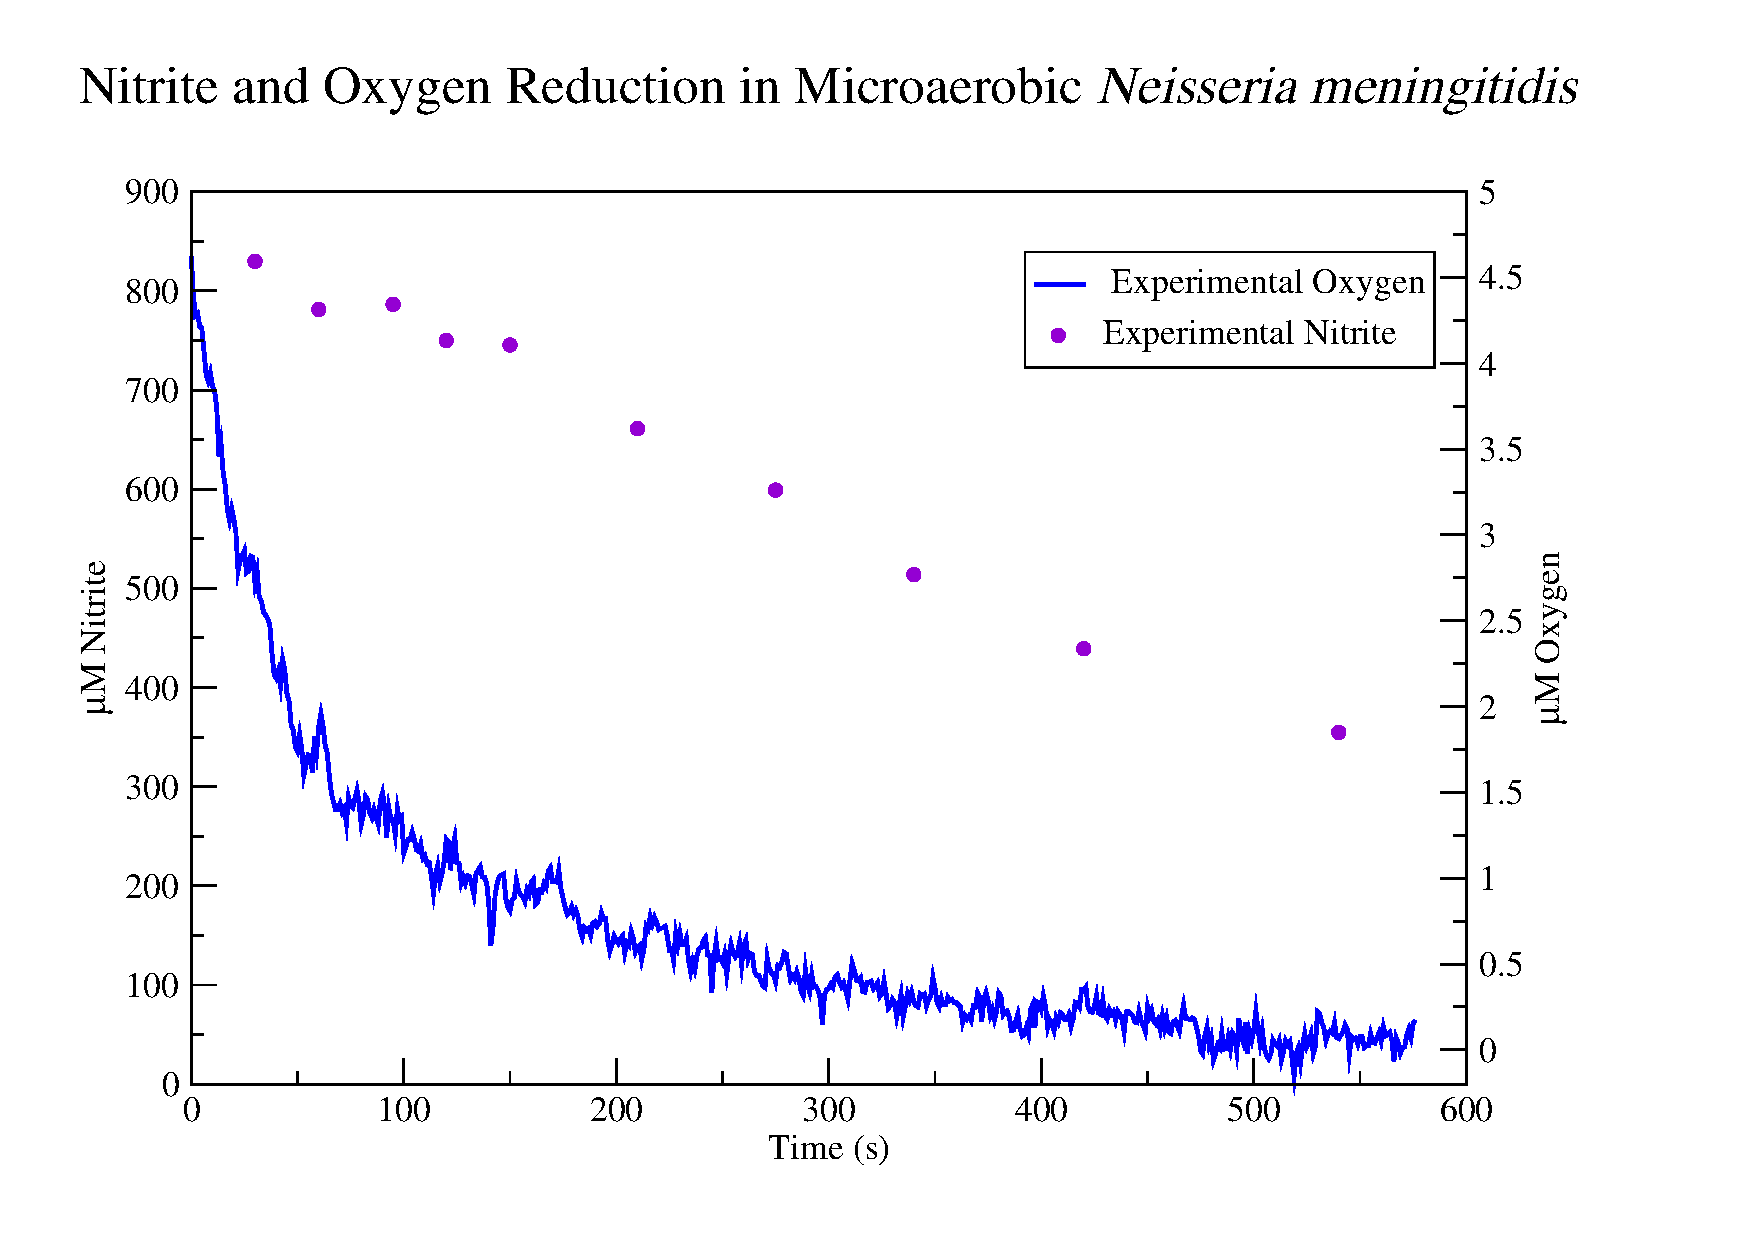
\includegraphics[height=10cm]{./07-nitritereduction/data/dataset1.pdf}
 % dataset1.pdf: 842x595 pixel, 72dpi, 29.70x20.99 cm, bb=0 0 842 595
 \caption[Nitrite Reduction in \Nsm{}]{{\bf Nitrite Reduction in \Nsm{}.} This dataset shows the effect on oxygen respiration of nitrite respiration as nitric oxide is produced. This culture is an $nsrR^-$ mutant which is expressing AniA and NorB in an essentially constitutive manner.
 \label{fig:nitriteds1}}
\end{figure}

\begin{figure}[tbp]
 \centering
 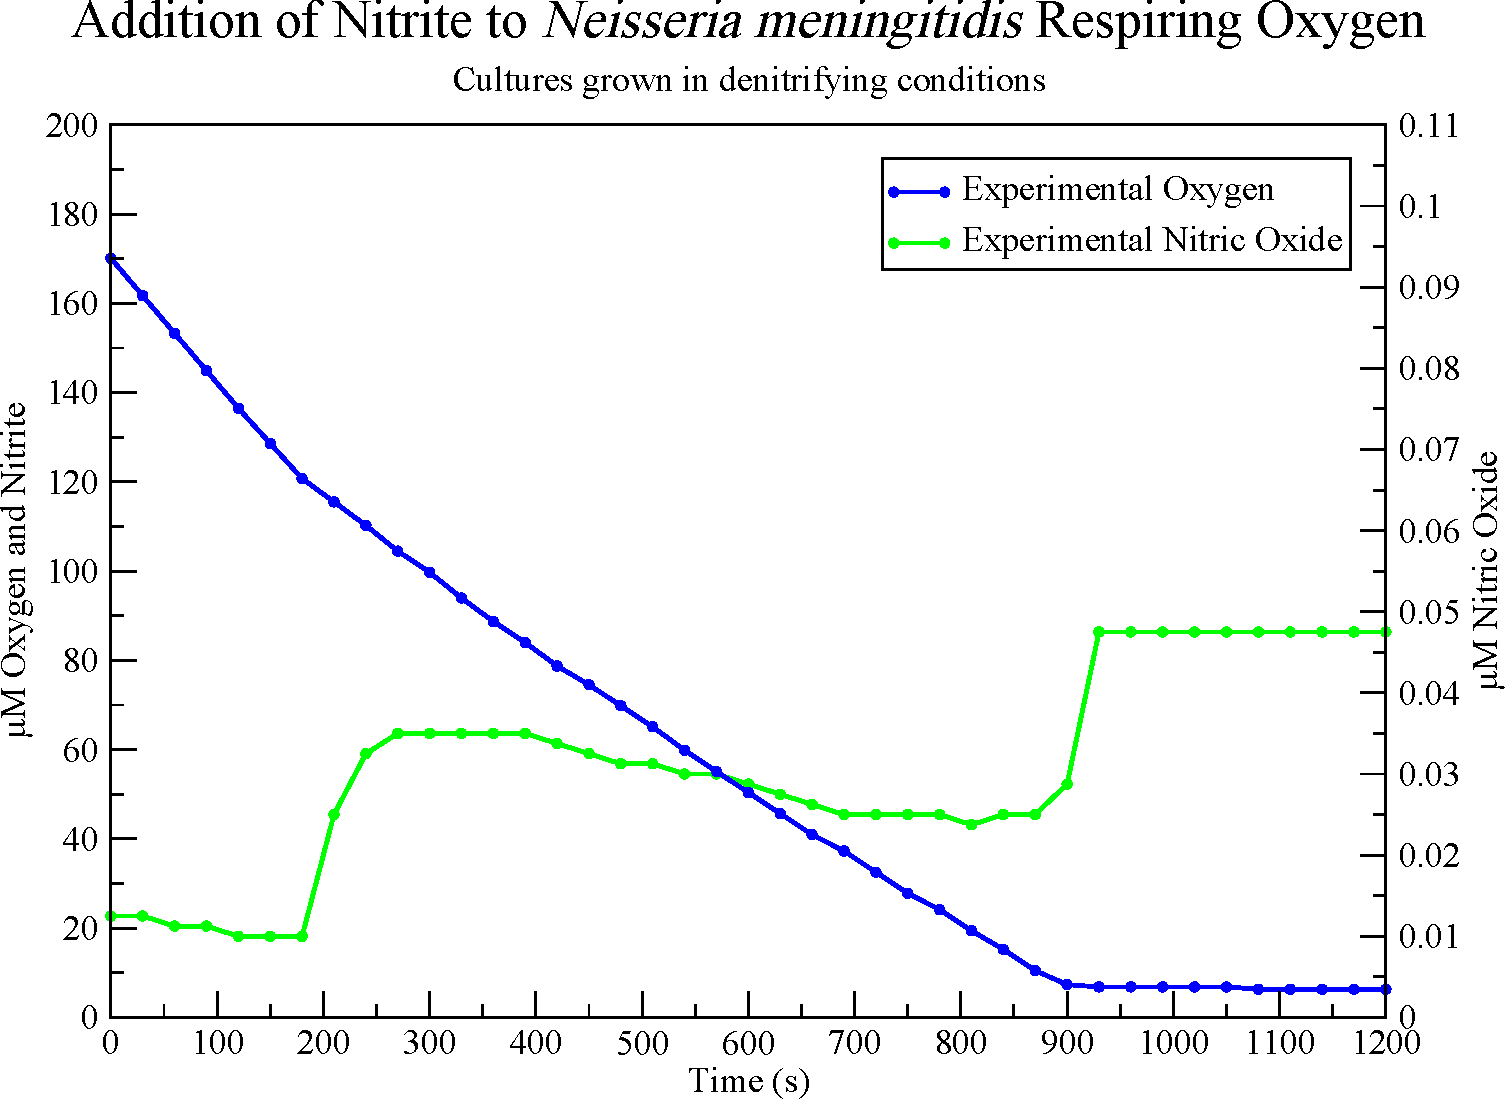
\includegraphics[height=10cm]{./07-nitritereduction/data/dataset2.pdf}
 % dataset1.pdf: 842x595 pixel, 72dpi, 29.70x20.99 cm, bb=0 0 842 595
 \caption[Nitrite Reduction in \Nsm{}]{{\bf Nitrite Reduction in \Nsm{}.} This dataset shows the effect of nitrite addition to an aerobically respiring culture. Nitrite is added at 200s. Oxygen and Nitric Oxide data-points are recorded with much less frequency than in previous datasets hence the inclusion of dots on the plot.
 \label{fig:nitriteds2}}
\end{figure}

\subsection{Prior Probability Distributions}

As described previously all parameters must have an associated prior probability distribution. The posterior probability distributions from Chapter \ref{chap:noreduction} were used as prior probability distributions in this chapter. Where new parameters were introduced, the distributions were generated based on published literature values which are noted in Chapter \ref{chap:model}. When using literature values the prior probability distributions were generated according to the same scheme as in Chapter \ref{chap:oxygenreduction}. The values required to create idealised lognormal probability distributions for each parameters are shown in Table \ref{tab:nitrite_prior_table}.

\begin{table}[ht]%needs to be 'here' as section is short
\renewcommand{\arraystretch}{1.5}
\begin{center}
\begin{tabular}{cccc|cccc}
\toprule
\textbf{Parameter} && ${\bar{x}}$ & $\sigma$ & \textbf{Parameter} && ${\bar{x}}$ & $\sigma$\\
\midrule
$k_1$ && 417.88 & 31.172 & g && 0.857 & 0.086\\
$k_3$ && 4.65 & 0.619 & f && 8.398 & 1.237\\
$l_1$ && 13.12 & 8.321 & $\gamma$ && 0.00014 & $4.67\times 10^{-6}$\\
$l_3$ && 0.058 & 0.021 & Q && 7.06 & 1.317\\
$m_1$ && 1 & 1 & X && 27.45 & 12.08\\
$m_3$ && 4.8 & 0.2 & A && 0.137 & 0.048\\
$k_5$ && 1741.8 & 1822.0 & B && 0.137 & 0.048\\
$k_6$ && 1.076 & 1.473 & C && 0.071 & 0.029\\
$\beta$ && 0.00014 & $4.67\times 10^{-6}$\\
\bottomrule
\end{tabular}
\end{center}
\caption[Prior Probability Table]{{\bf Prior Probability Table} This table shows the prior means and standard deviations used to create lognormal distributions to be used as the prior probability distributions.
\label{tab:nitrite_prior_table}}
\end{table}

The initial probability distributions used to start the Monte-Carlo runs are shown in Figure \ref{fig:nitrite_priors1}.

\begin{figure}[tbp]
 \centering
 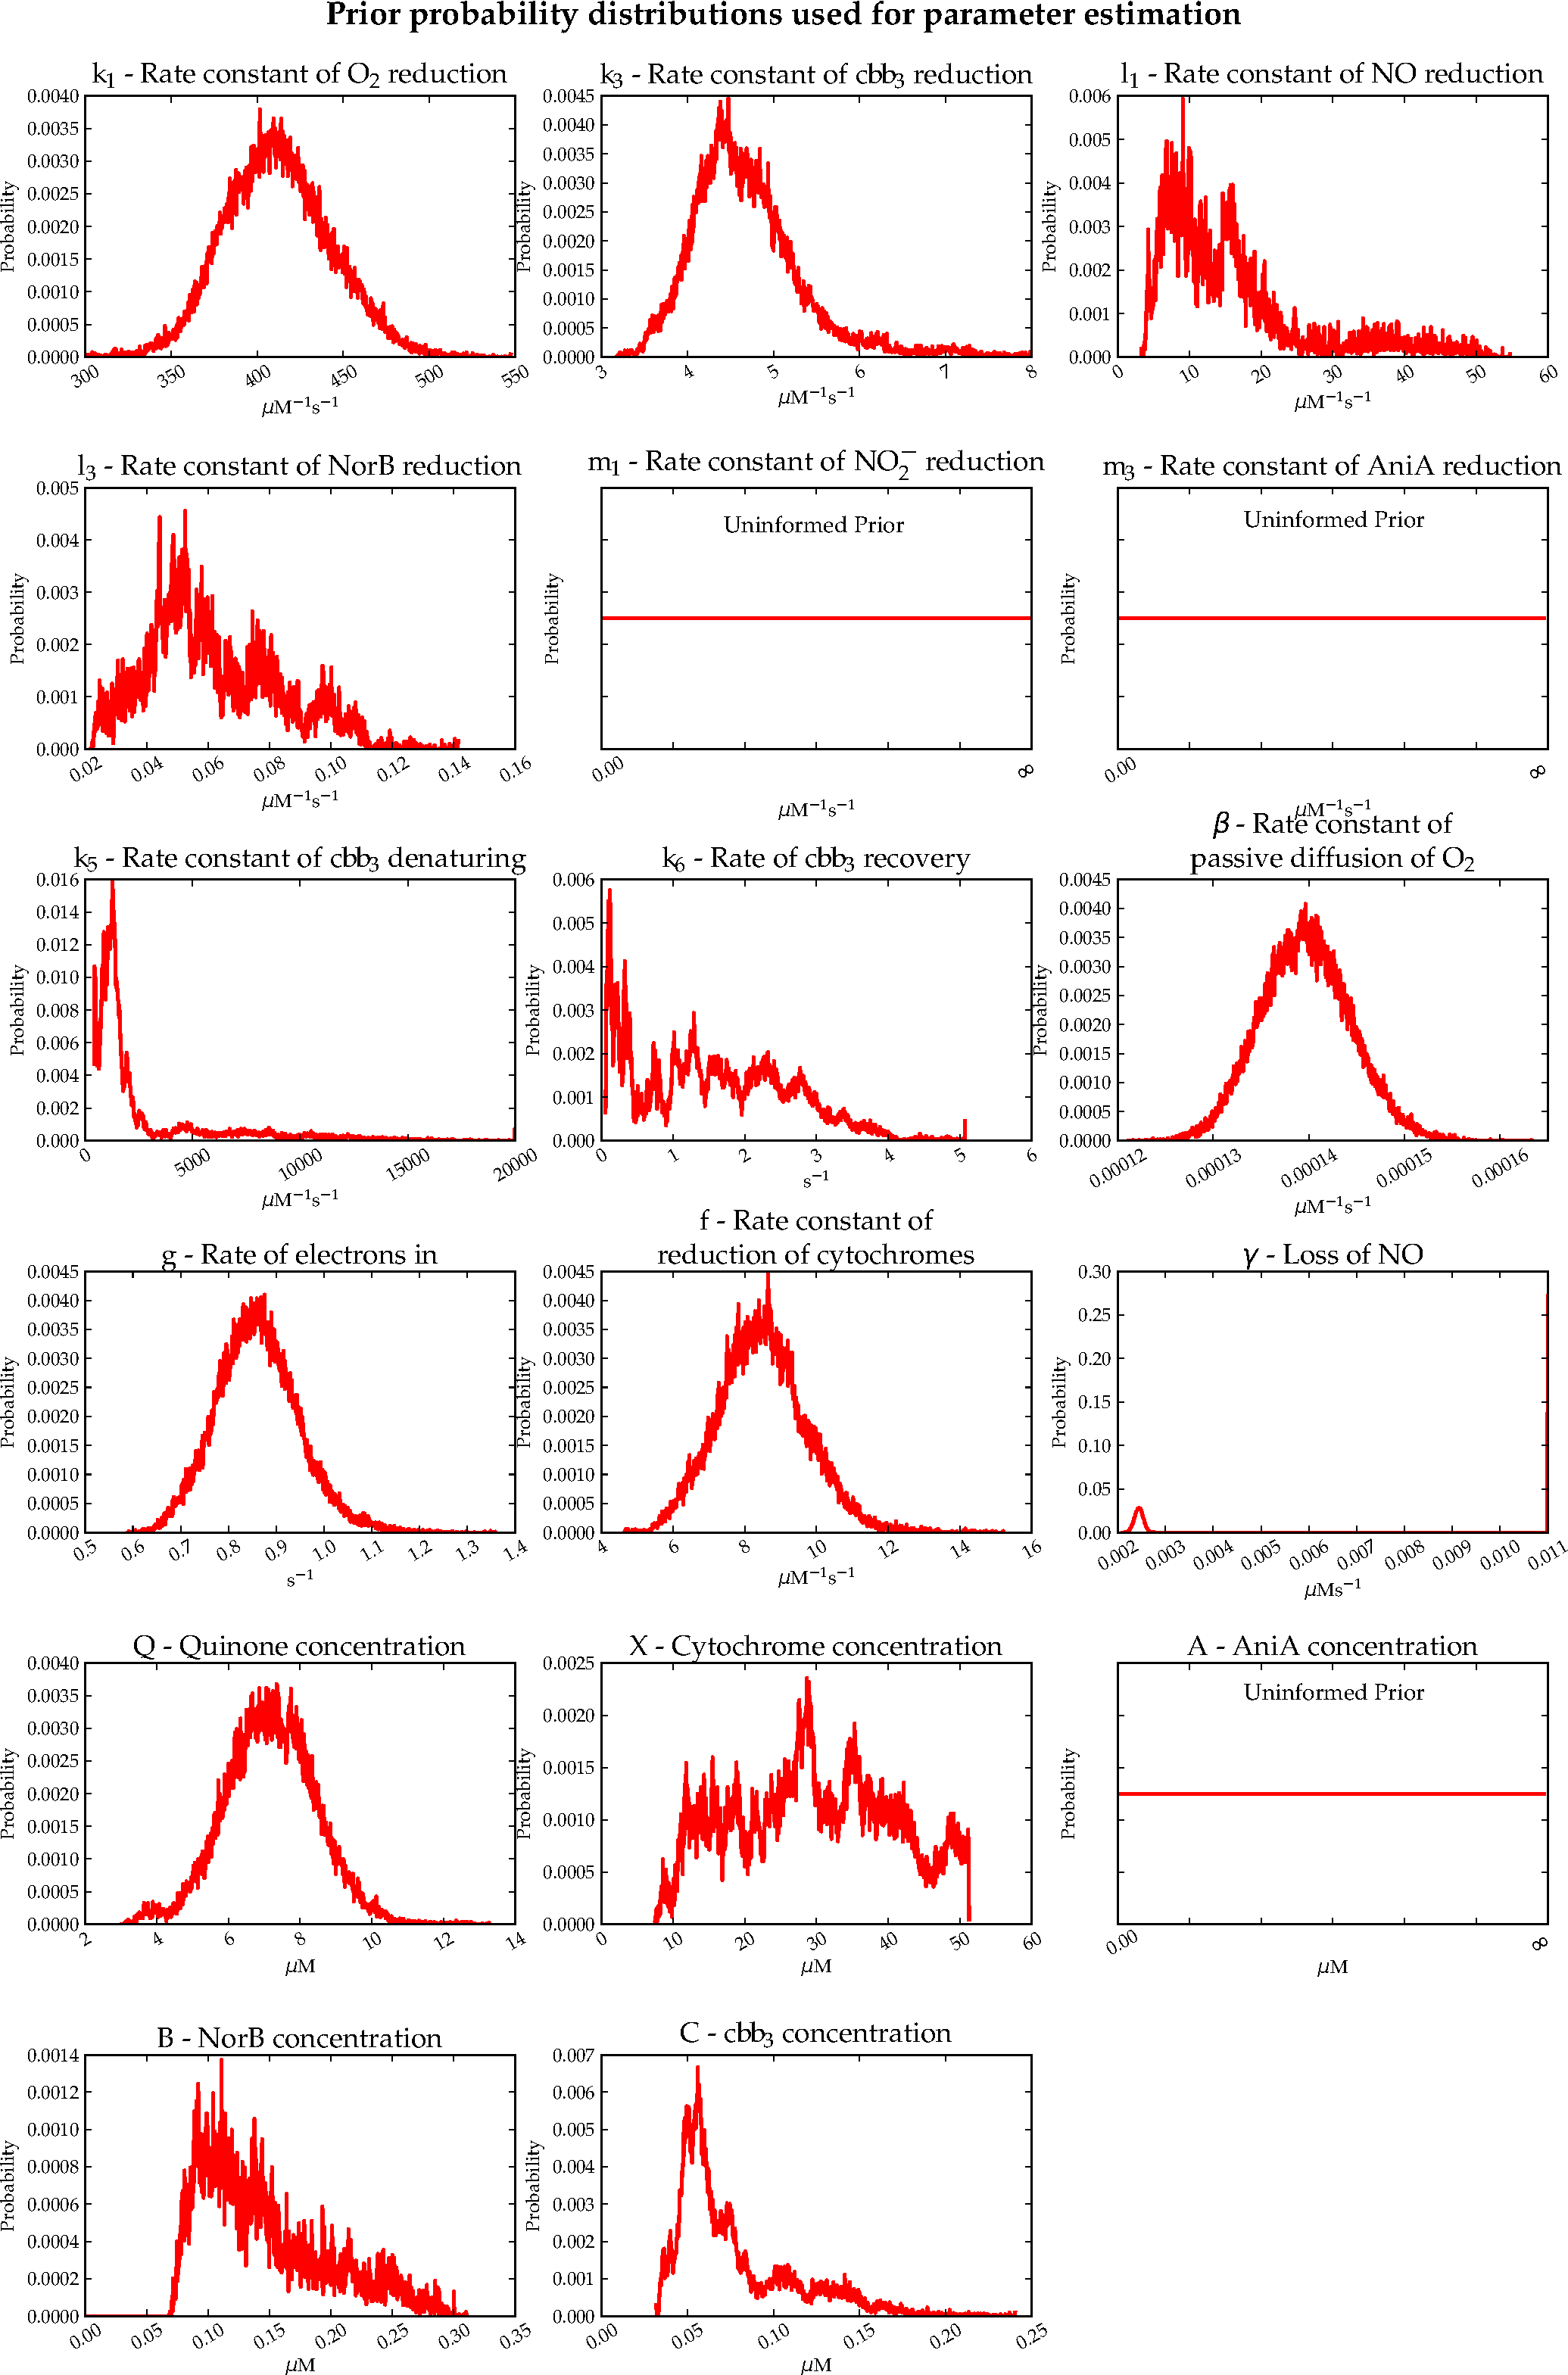
\includegraphics[width=15cm, trim=0cm 4.1cm 0cm 1cm, clip=true]{./07-nitritereduction/data/priors1.pdf}
 % priors.pdf: 1008x1008 pixel, 72dpi, 35.56x35.56 cm, bb=0 0 1008 1008
 \caption[Prior probability distributions for microaerobic oxygen and nitrite reduction]{{\bf Prior probability distributions for microaerobic oxygen and nitrite reduction}. These are the probability distributions used as priors by the parameter estimation algorithm.
 \label{fig:nitrite_priors1}}
\end{figure}
\afterpage{\clearpage}

\subsection{Parameter Estimation Results}
The parameter estimation process was run in the same fashion as that described in Chapters \ref{chap:oxygenreduction} \& \ref{chap:noreduction}. The 2 experimental datasets were run 20 times (each) for 20,000 iterations using the prior probability distributions shown in Figure \ref{fig:nitrite_priors1}. The solved output from datasets 1 and 2 are shown in Figures \ref{fig:nitrite_ds1_solved1} and \ref{fig:nitrite_ds2_solved1} respectively. Given the apparent poor fitting of the solved outputs shown in both of these figures, plots of the redox states for both of these datasets are shown in Figures \ref{fig:nitrite_ds1_redox1} and \ref{fig:nitrite_ds2_redox1}.

\begin{figure}[tbp]
 \centering
 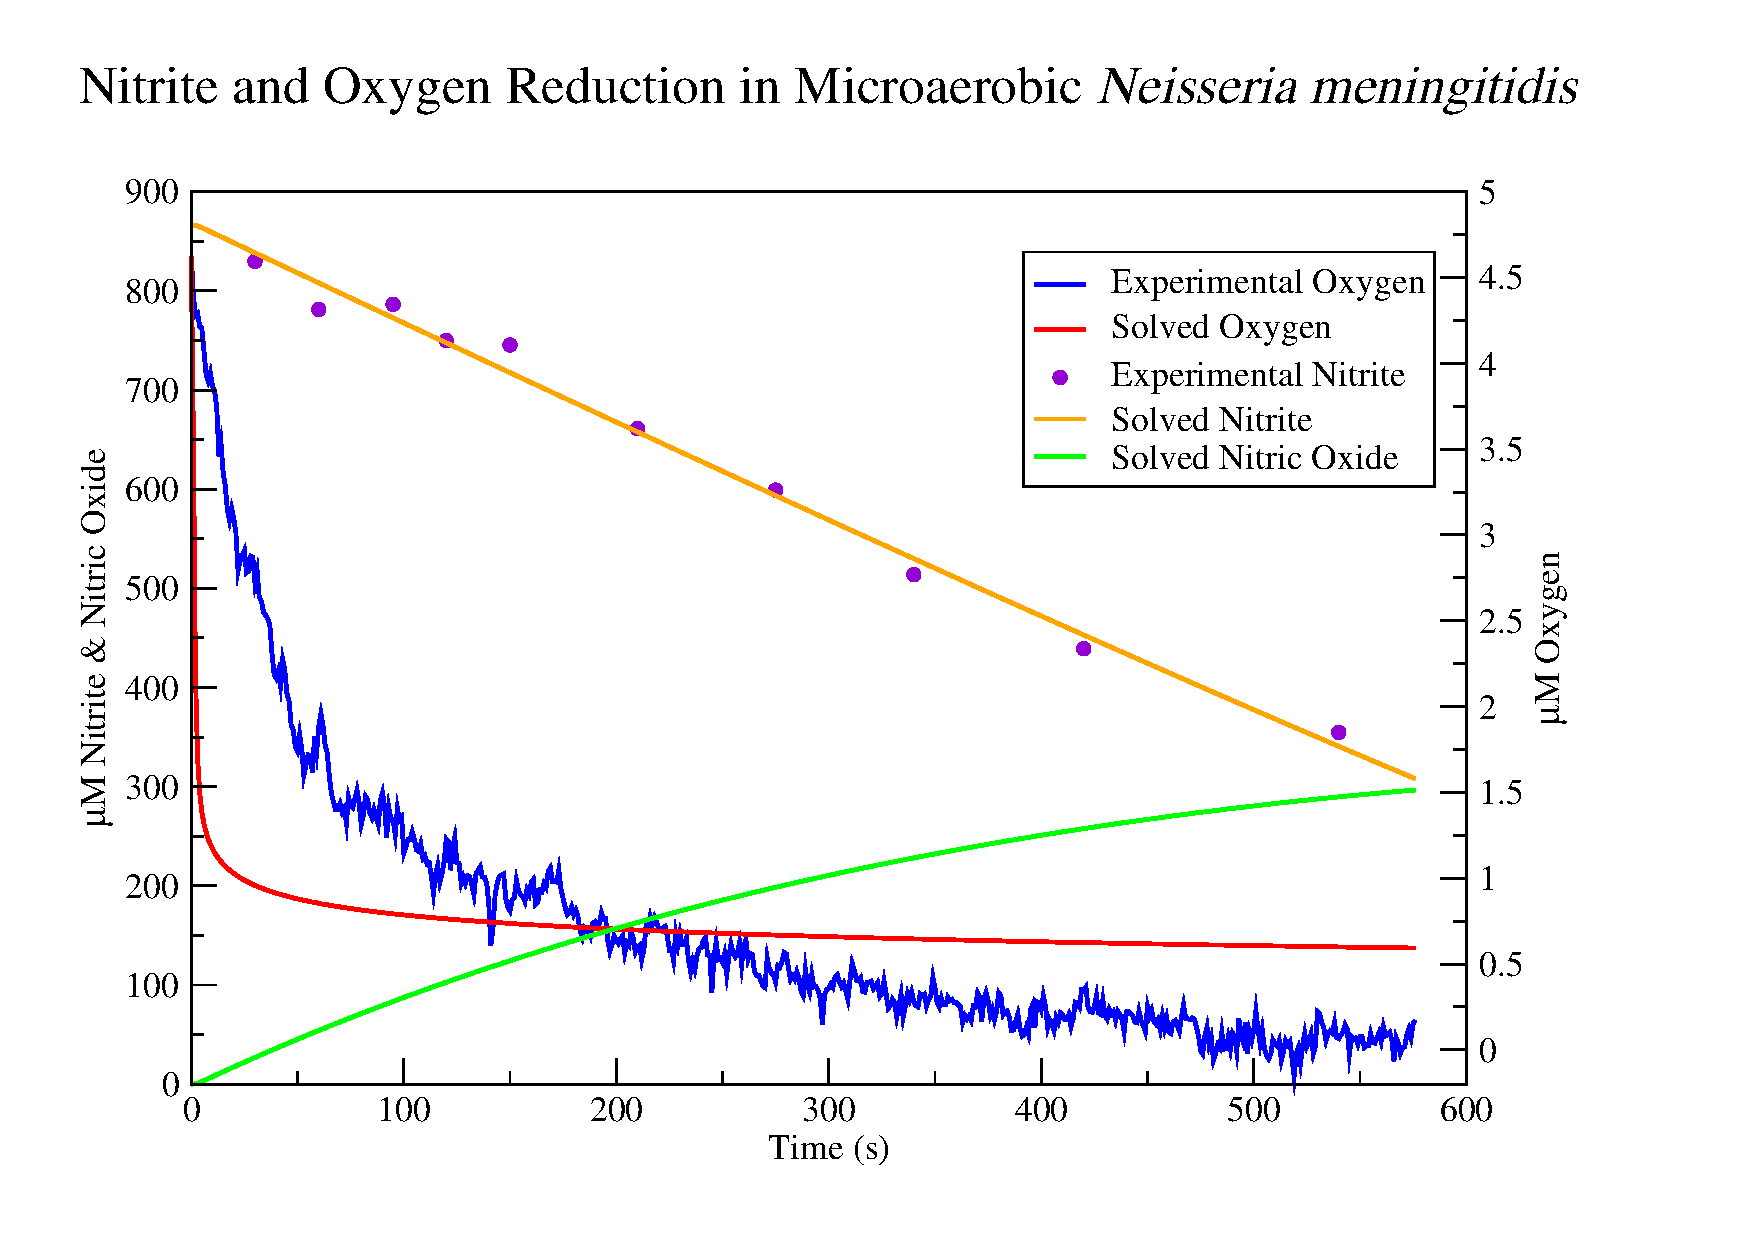
\includegraphics[height=10cm, clip=true]{./07-nitritereduction/data/dataset1-1.pdf}
 % dataset1-1.pdf: 842x595 pixel, 72dpi, 29.70x20.99 cm, bb=0 0 842 595
 \caption[Solved Nitrite Reduction in \Nsm{}]{{\bf Solved Nitrite Reduction in \Nsm{}}. This figure shows the first attempt at fitting the model to experimental data. Nitrite reduction is being modelled well, whereas oxygen reduction is being modelled quite poorly as the solved data shows to high a rate of oxygen reduction. Nitric oxide is solved purely as a product of nitrite reduction and is not compared to any experimental data.
  \label{fig:nitrite_ds1_solved1}}
\end{figure}

The solved data shown in Figure \ref{fig:nitrite_ds1_solved1} doesn't fit particularly well to the experimental data. Nitrite reduction appears to be modelled well as it is a simple linear reduction. Oxygen reduction however is modelled very poorly. The initial rate of oxygen reduction is too high, and the reduction in rate is too fast. The halting of oxygen reduction is due to the amount of nitric oxide being produced by the reduction of nitrite. This level of nitric oxide quickly inhibits the \cbbthree{} totally as can be seen by the large level of nitric oxide concentration in Figure \ref{fig:nitrite_ds1_solved1} and in the redox plot in Figure \ref{fig:nitrite_ds1_redox1}. The redox plots show that essentially all the electrons in the system are flowing to the nitrite reduction pathway. Nitric oxide is progressing as fast as possible based on the electron flow into NorB. NorB stays in a permanently oxidised state suggesting that the reduction activity of NorB is faster than the rate of reduction of NorB itself. The level of NorB is also not easily modelled correctly using this data as no information is available about the actual levels of nitric oxide being produced during nitrite reduction.

\begin{figure}[tbp]
 \centering
 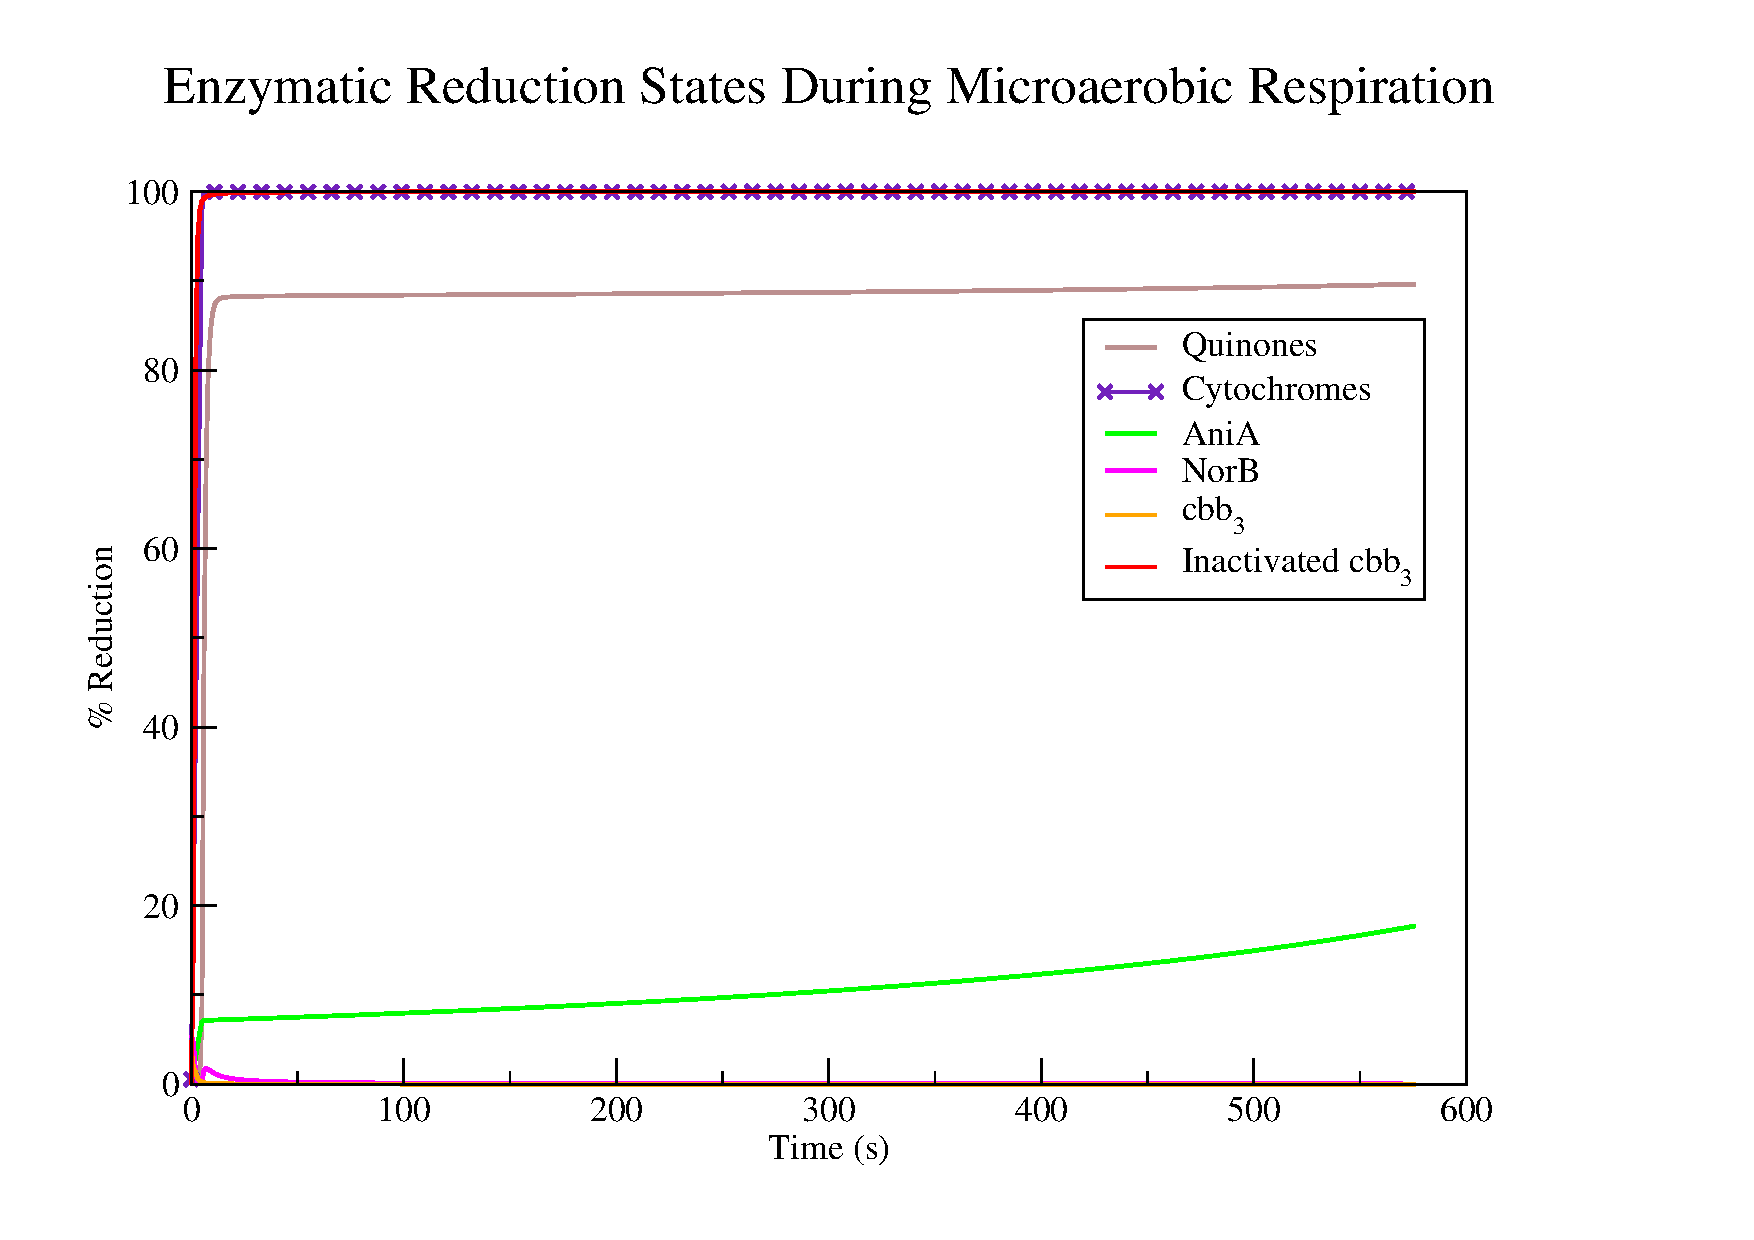
\includegraphics[height=10cm, clip=true]{./07-nitritereduction/data/dataset1redox-1.pdf}
 % dataset1redox-1.pdf: 842x595 pixel, 72dpi, 29.70x20.99 cm, bb=0 0 842 595
 \caption[Reduction States During Nitrite Reduction]{{\bf Reduction States During Nitrite Reduction}. This figure shows how the reduction states of the enzymes involved in nitrite reduction change during respiration.
  \label{fig:nitrite_ds1_redox1}}
\end{figure}

The solved data in Figure \ref{fig:nitrite_ds2_solved1} appears to fit oxygen reduction quite well but fails to fit nitric oxide reduction almost entirely. The most significant feature, that nitric oxide should increase when oxygen reduction ceases is missing. The redox state plot in Figure \ref{fig:nitrite_ds2_redox1} suggests the reason for the lack of this feature. The cytochromes appear to be in a completely reduced state shortly after the start of the simulation. This permanently reduced state means that when oxygen reduction ceases there is essentially no difference to the flow of electrons to either NorB or AniA. This suggests that parameters $g$ and $f$, the reduction of cytochromes and the reduction of the quinone pool are too high, leading to the permanent reduction of both those components. The nitrite levels are equally difficult to model as nitric oxide in the previous dataset as the levels are unknown.

\begin{figure}[tbp]
 \centering
 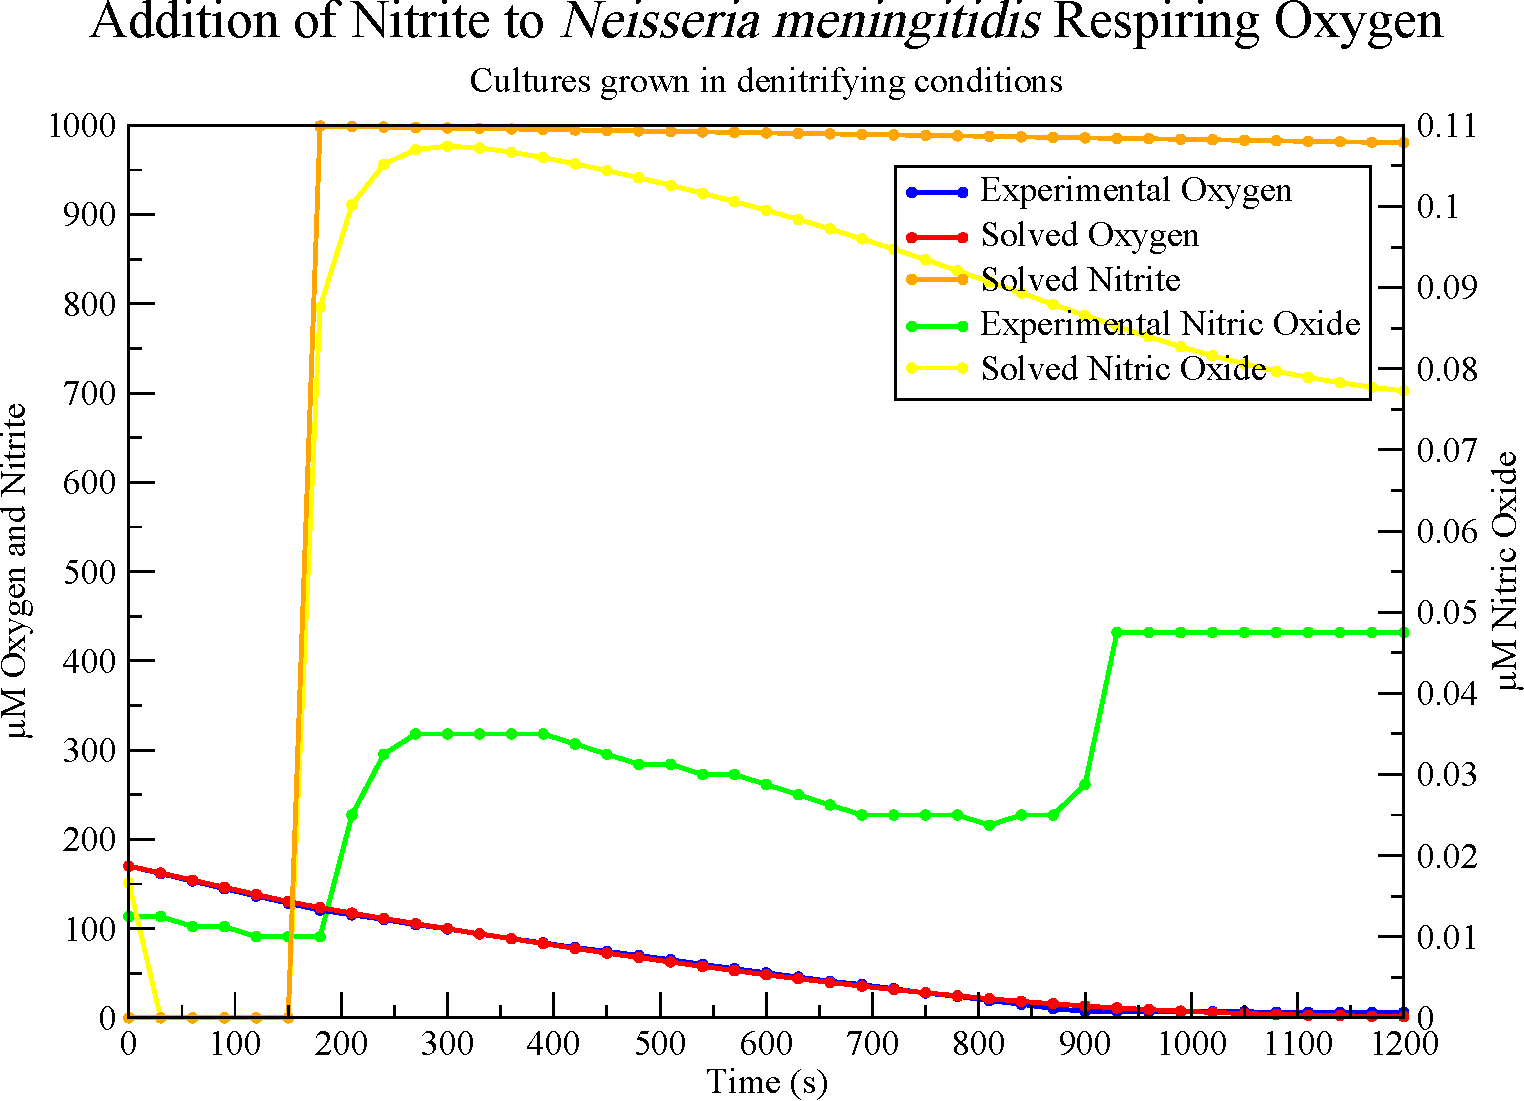
\includegraphics[height=10cm, clip=true]{./07-nitritereduction/data/dataset2-1.pdf}
 % dataset2-1.pdf: 842x595 pixel, 72dpi, 29.70x20.99 cm, bb=0 0 842 595
 \caption[Effect of Nitrite Addition on Aerobically Respiring Cultures]{{\bf Effect of Nitrite Addition on Aerobically Respiring Cultures}. This figure shows the first attempt at fitting the model to experimental data. Oxygen respiration appears appears to be modelled quite well, but nitric oxide is being modelled particularly badly. The most significant feature of the nitric oxide dataset is absent in the solved data.
  \label{fig:nitrite_ds2_solved1}}
\end{figure}

\begin{figure}[tbp]
 \centering
 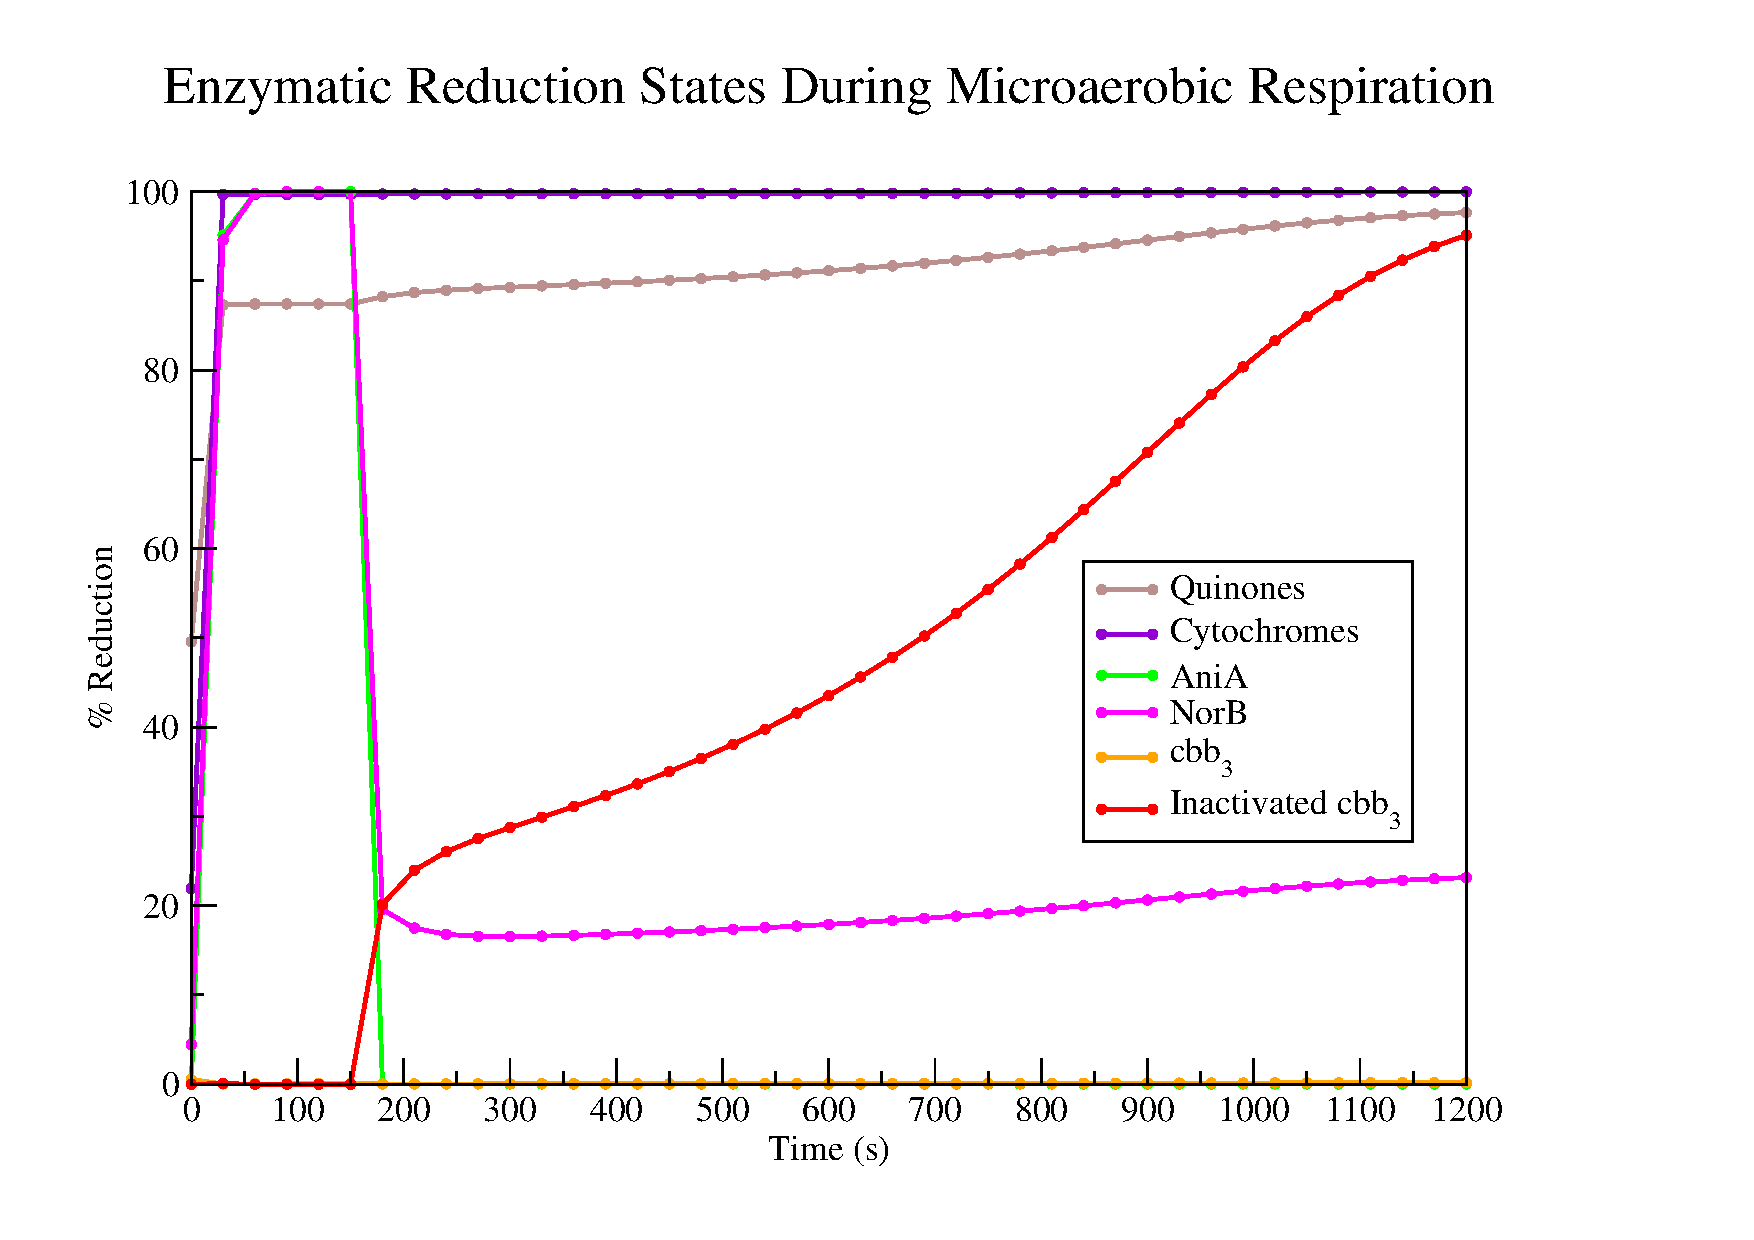
\includegraphics[height=10cm, clip=true]{./07-nitritereduction/data/dataset2redox-1.pdf}
 % dataset2redox-1.pdf: 842x595 pixel, 72dpi, 29.70x20.99 cm, bb=0 0 842 595
 \caption[Reduction States During Nitrite Reduction]{{\bf Reduction States During Nitrite Reduction}. This figure shows how the reduction states of the enzymes involved in nitrite reduction change during respiration.
  \label{fig:nitrite_ds2_redox1}}
\end{figure}

The posterior probability distributions for the above results are not shown here as they do not provide any useful information at this point.

\subsection{Second Parameter Estimation Results}
A second attempt was made to try and better fit the solved data to the experimental data by adapting the priors for dataset 2 using knowledge from the previous parameter estimation attempt. The prior probability distributions for dataset 2 were altered such that the means of $f$ and $g$ were reduced 10 fold, and the distributions were broadened significantly. Additionally the $m_3$ rate constant prior distribution was set correctly. The other distributions were left unchanged. The new prior probability distributions are shown in Figure \ref{fig:nitrite_priors2}.

\begin{figure}[tbp]
 \centering
 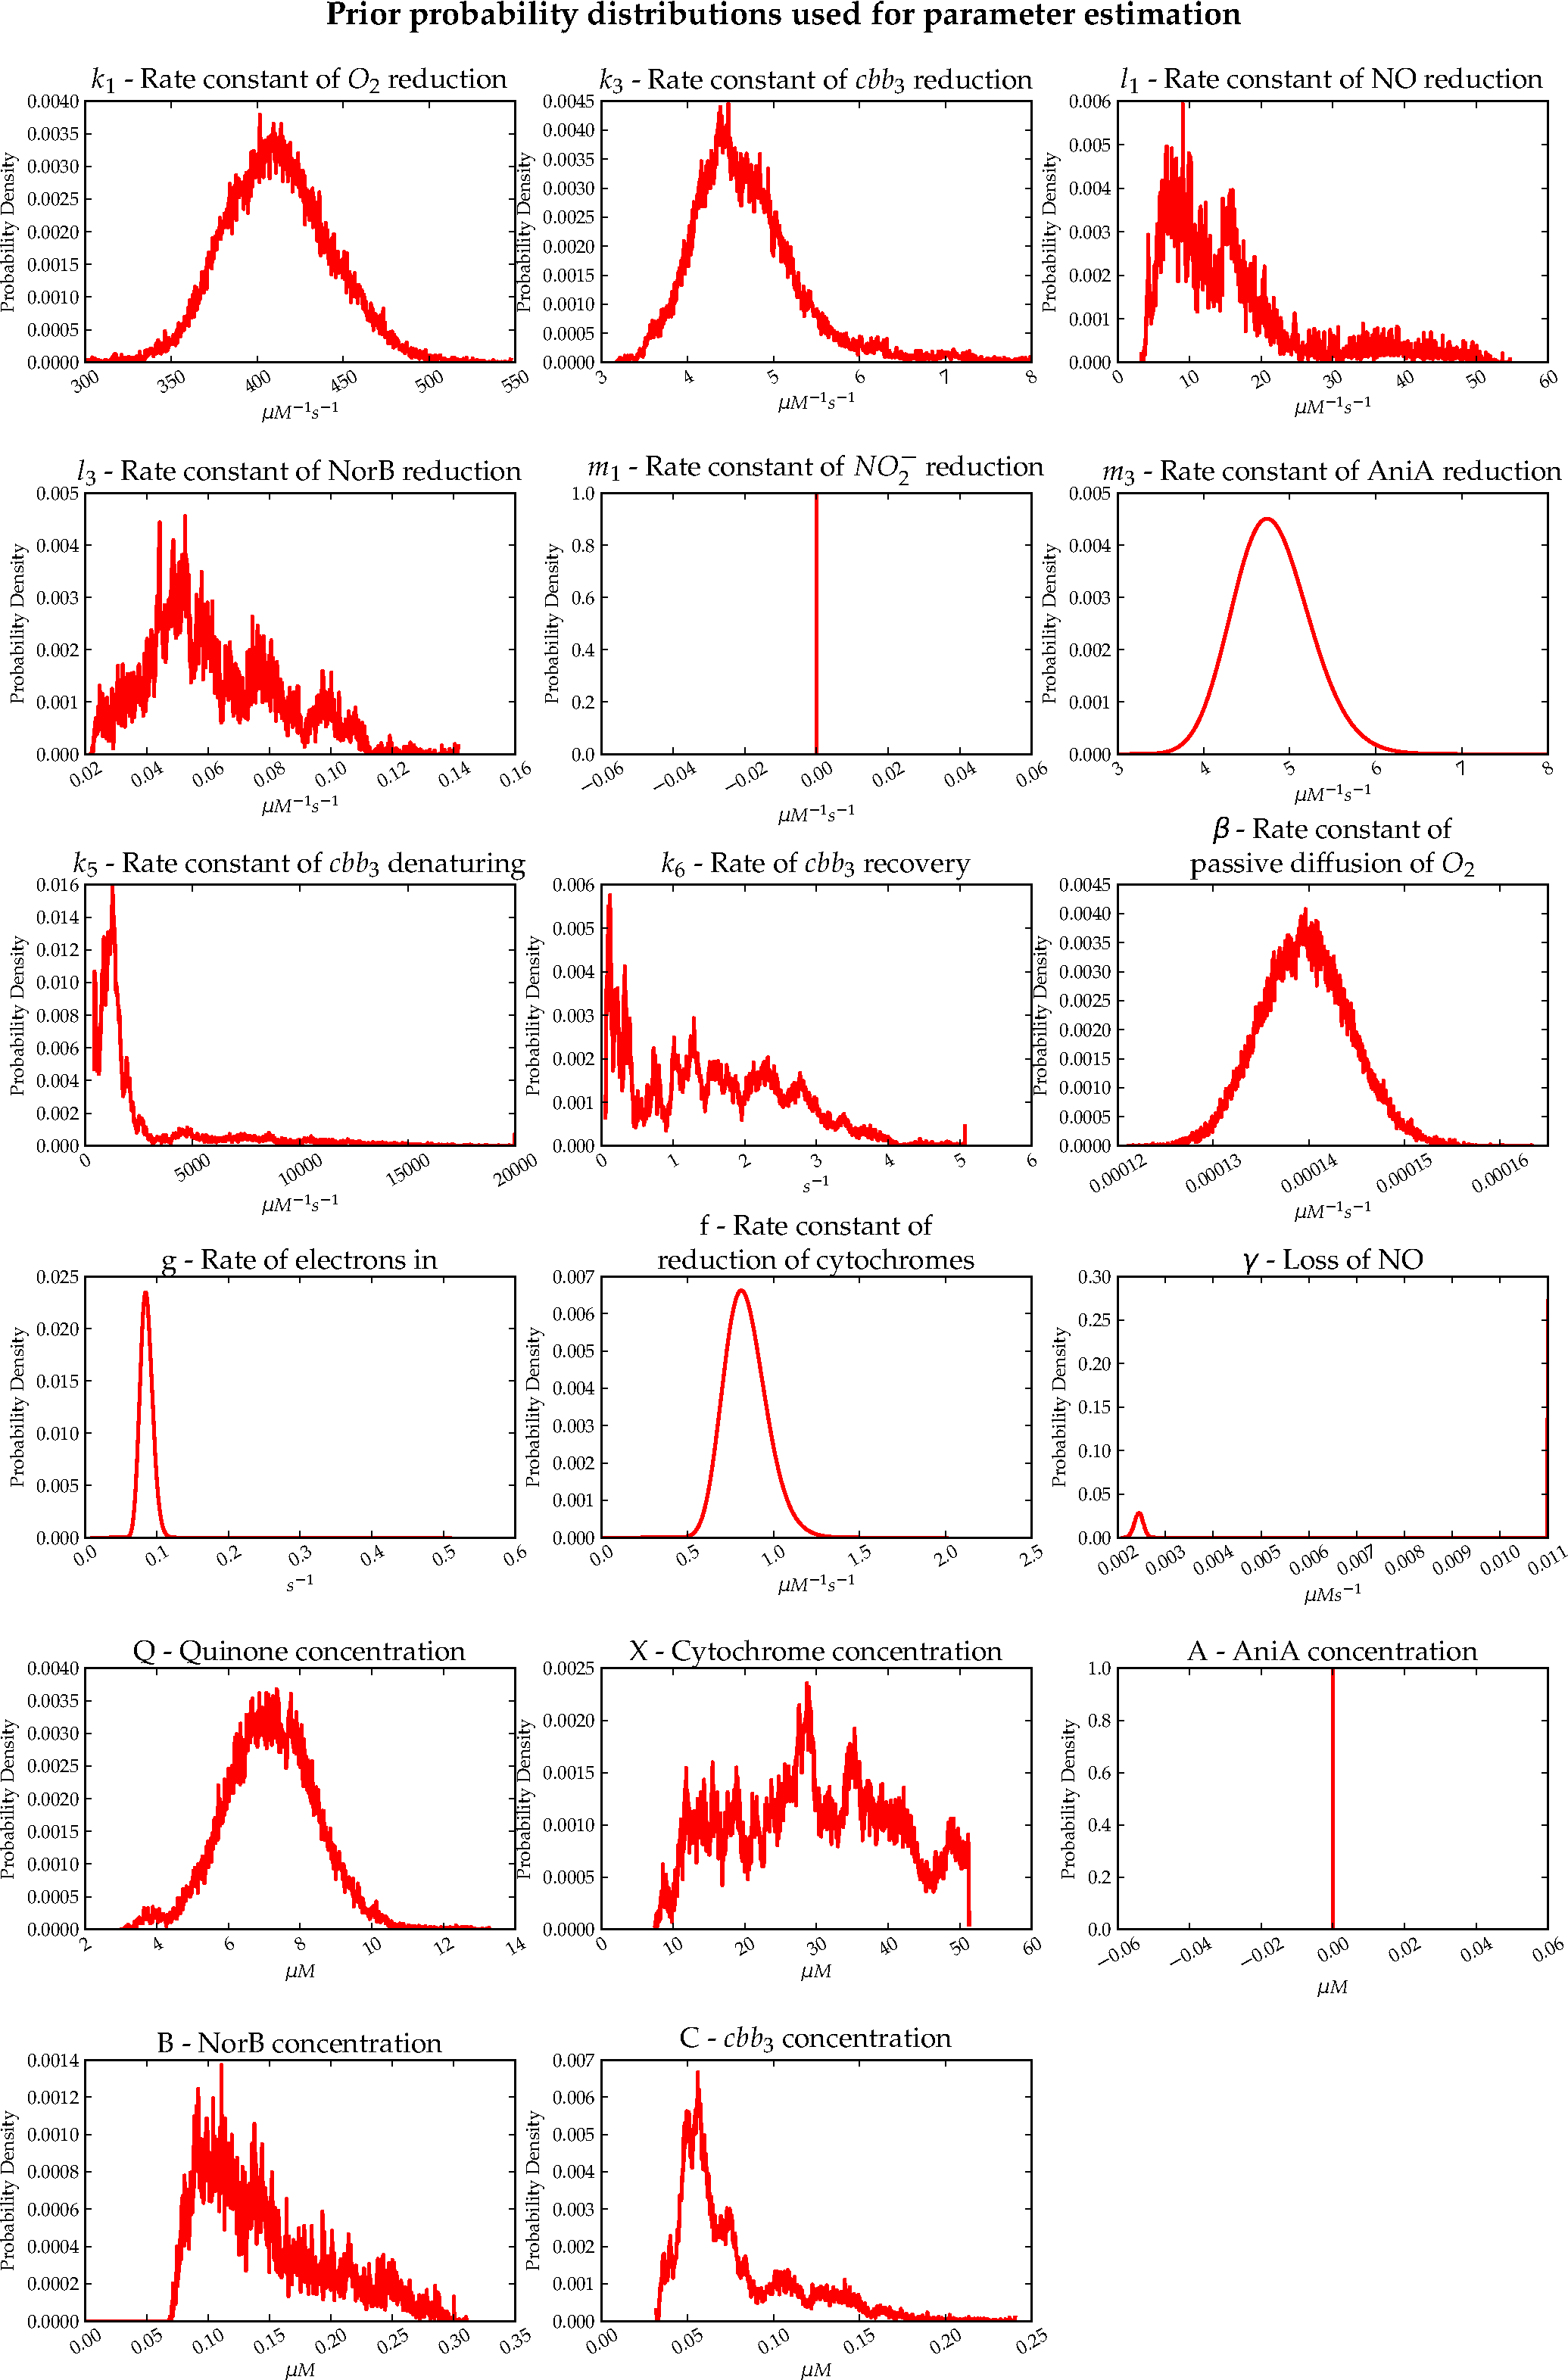
\includegraphics[width=15cm, trim=0cm 0cm 0cm 0cm, clip=true]{./07-nitritereduction/data/priors2.pdf}
 % priors.pdf: 1008x1008 pixel, 72dpi, 35.56x35.56 cm, bb=0 0 1008 1008
 \caption[Prior probability distributions for microaerobic oxygen and nitrite reduction]{{\bf Prior probability distributions for microaerobic oxygen and nitrite reduction}. These are the modified probability distributions used as priors by the parameter estimation algorithm.
 \label{fig:nitrite_priors2}}
\end{figure}
\afterpage{\clearpage}

The new prior probability distributions proved to be difficult for the parameter estimation system to use, as out of 10 runs only 2 produced reasonable fitted data. One of these fits is shown in Figure \ref{fig:nitrite_ds2_solved2}. This shows a vastly improved fit over Figure \ref{fig:nitrite_ds2_solved1}. Oxygen is being modelled almost perfectly, and the major features of the nitric oxide data are also qualitatively present. In addition, the similarity between the oxygen reduction rates and nitrite reduction rates is corroborated by \citet{Rock2005} who showed that under denitrifying conditions nitrite reduction rate should roughly equal oxygen reduction rate.

\begin{figure}[tbp]
 \centering
 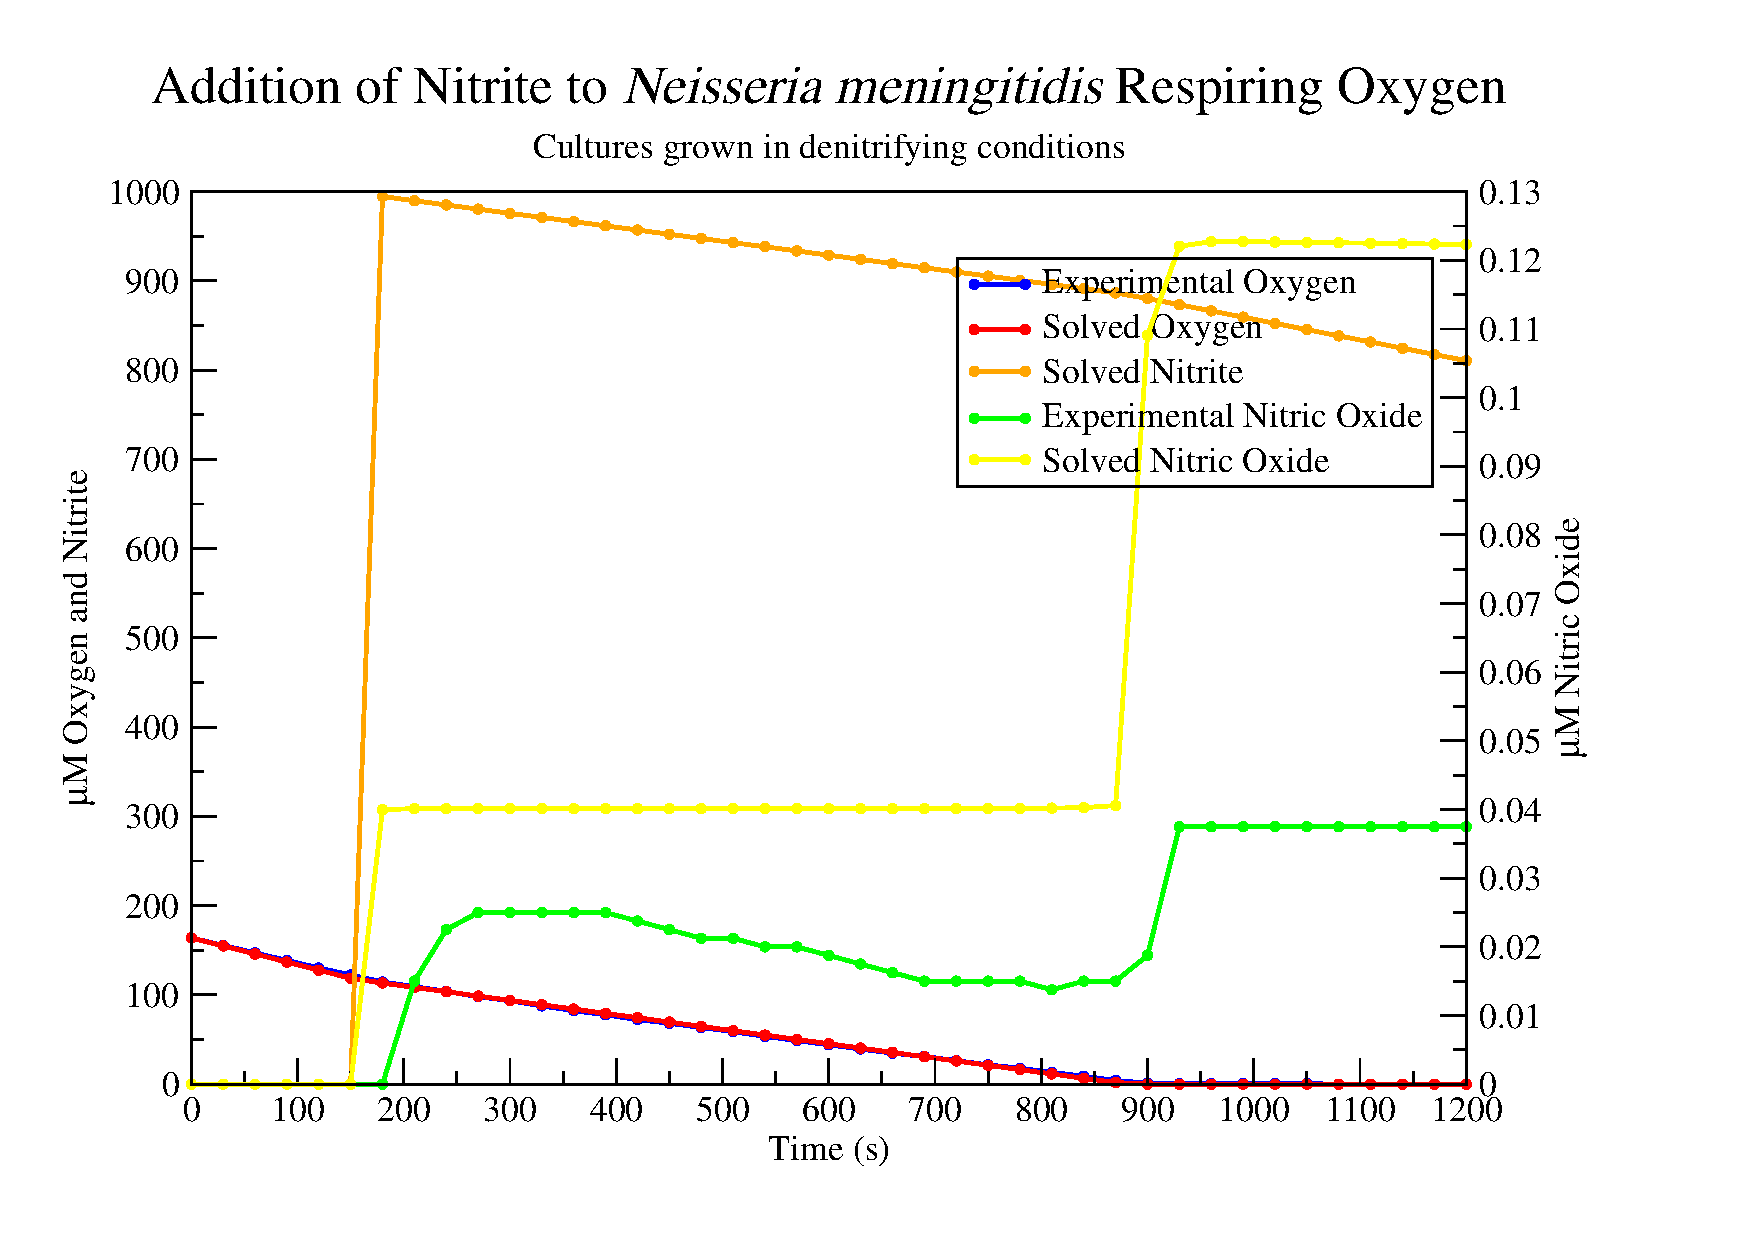
\includegraphics[height=10cm, clip=true]{./07-nitritereduction/data/dataset2-2.pdf}
 % dataset2redox-1.pdf: 842x595 pixel, 72dpi, 29.70x20.99 cm, bb=0 0 842 595
 \caption[Effect of Nitrite Addition on Aerobically Respiring Cultures]{{\bf Effect of Nitrite Addition on Aerobically Respiring Cultures}. This figure shows the second attempt at fitting the model to experimental data. Oxygen respiration appears appears to be modelled well. Nitric oxide production is being modelled well qualitatively, as the major features of the experimental data are present. Clearly though further rounds of parameter estimation are in order to improve the quantitative fit.
  \label{fig:nitrite_ds2_solved2}}
\end{figure}

The redox state plot shown in Figure \ref{fig:nitrite_ds2_redox2} shows how the change in substrate reduction has come about. The cytochrome and quinones are no longer in a permanently reduced state, and once oxygen is depleted NorB is able to access some of the electrons that were previously directed towards \cbbthree{}, causing the increase in nitric oxide concentration. Additionally the cytochrome pool increases its overall reduction state once oxygen is depleted, as one of the sinks for electrons is no longer active, this also has a small effect on the reduction state of AniA which increases due to the larger supply of upstream electrons available to it. The increase in electrons available to AniA also causes an increase in the rate of nitrite reduction. The more marked reduction state change of the quinone pool once the culture starts respiring nitrite is corroborated by data obtained by \citet{Otten1999} who found that the reduction state of the quinone pool in \textit{Paracoccus} differs between aerobic respiration and denitrification.

\begin{figure}[tbp]
 \centering
 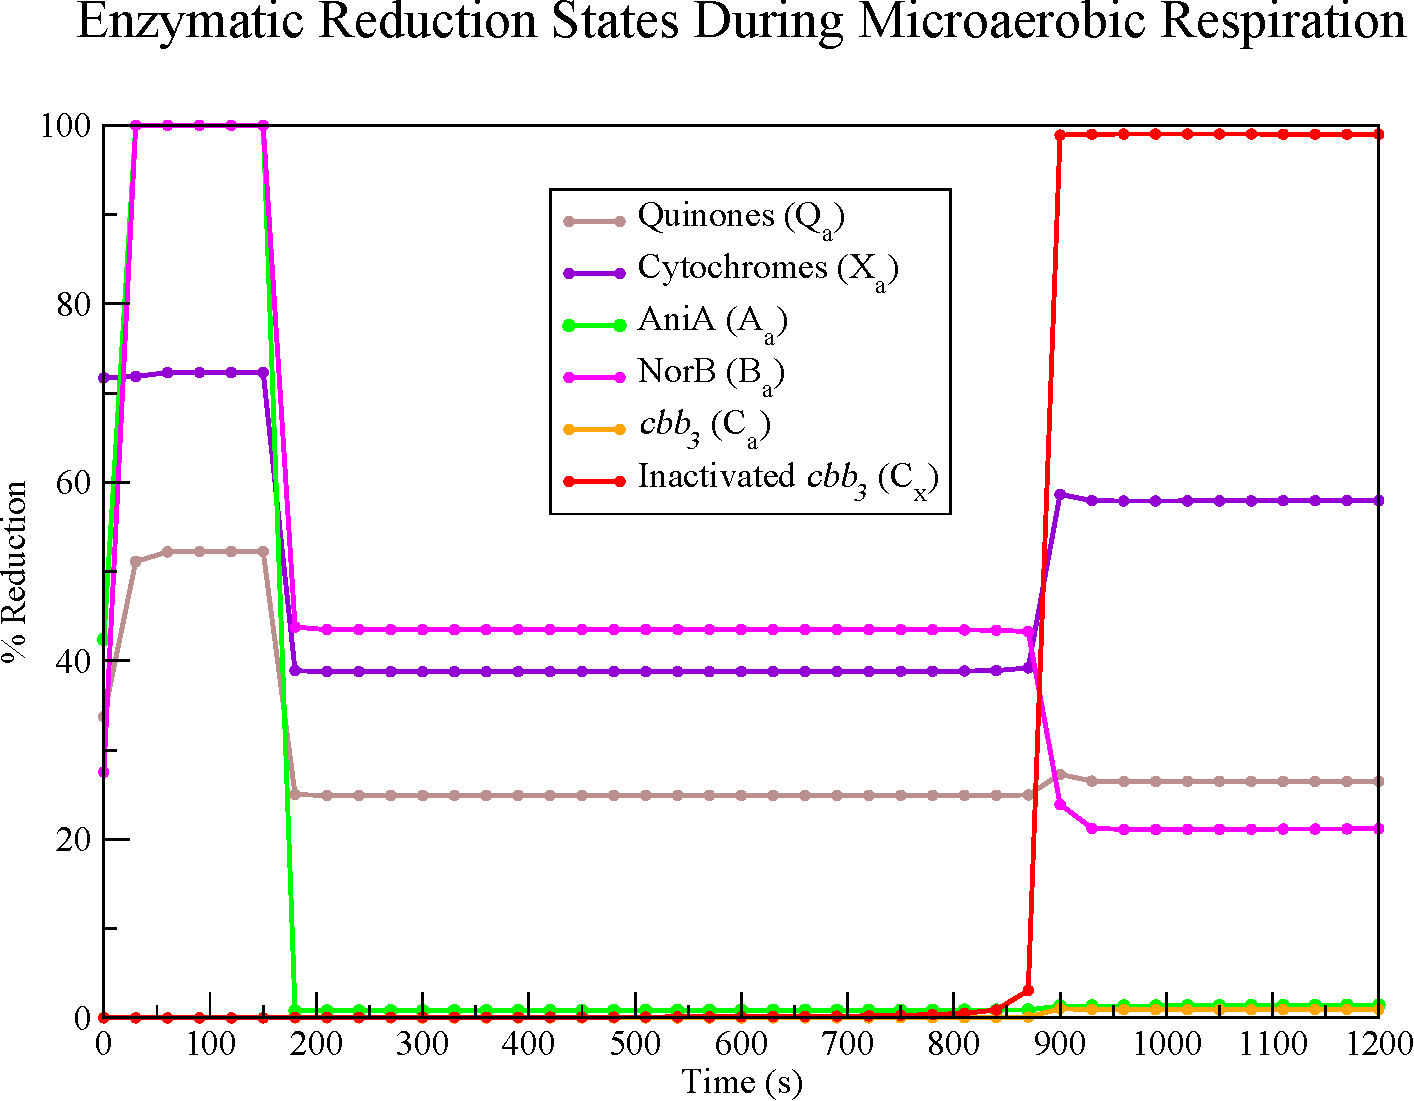
\includegraphics[height=10cm, clip=true]{./07-nitritereduction/data/dataset2redox-2.pdf}
 % dataset2redox-1.pdf: 842x595 pixel, 72dpi, 29.70x20.99 cm, bb=0 0 842 595
 \caption[Reduction States During Nitrite Reduction]{{\bf Reduction States During Nitrite Reduction}. This figure shows how the reduction states of the enzymes involved in nitrite reduction change during respiration.
  \label{fig:nitrite_ds2_redox2}}
\end{figure}

The posterior probability distributions generated from this second attempt at parameter estimation are shown in Figure \ref{fig:nitrite_posteriors1}. These were generated only from the two Markov Chains that produced simulation output that qualitatively matched the input data. The other Markov Chains settled on solved output which did not have the correct dataset features.

\begin{figure}[tbp]
 \centering
 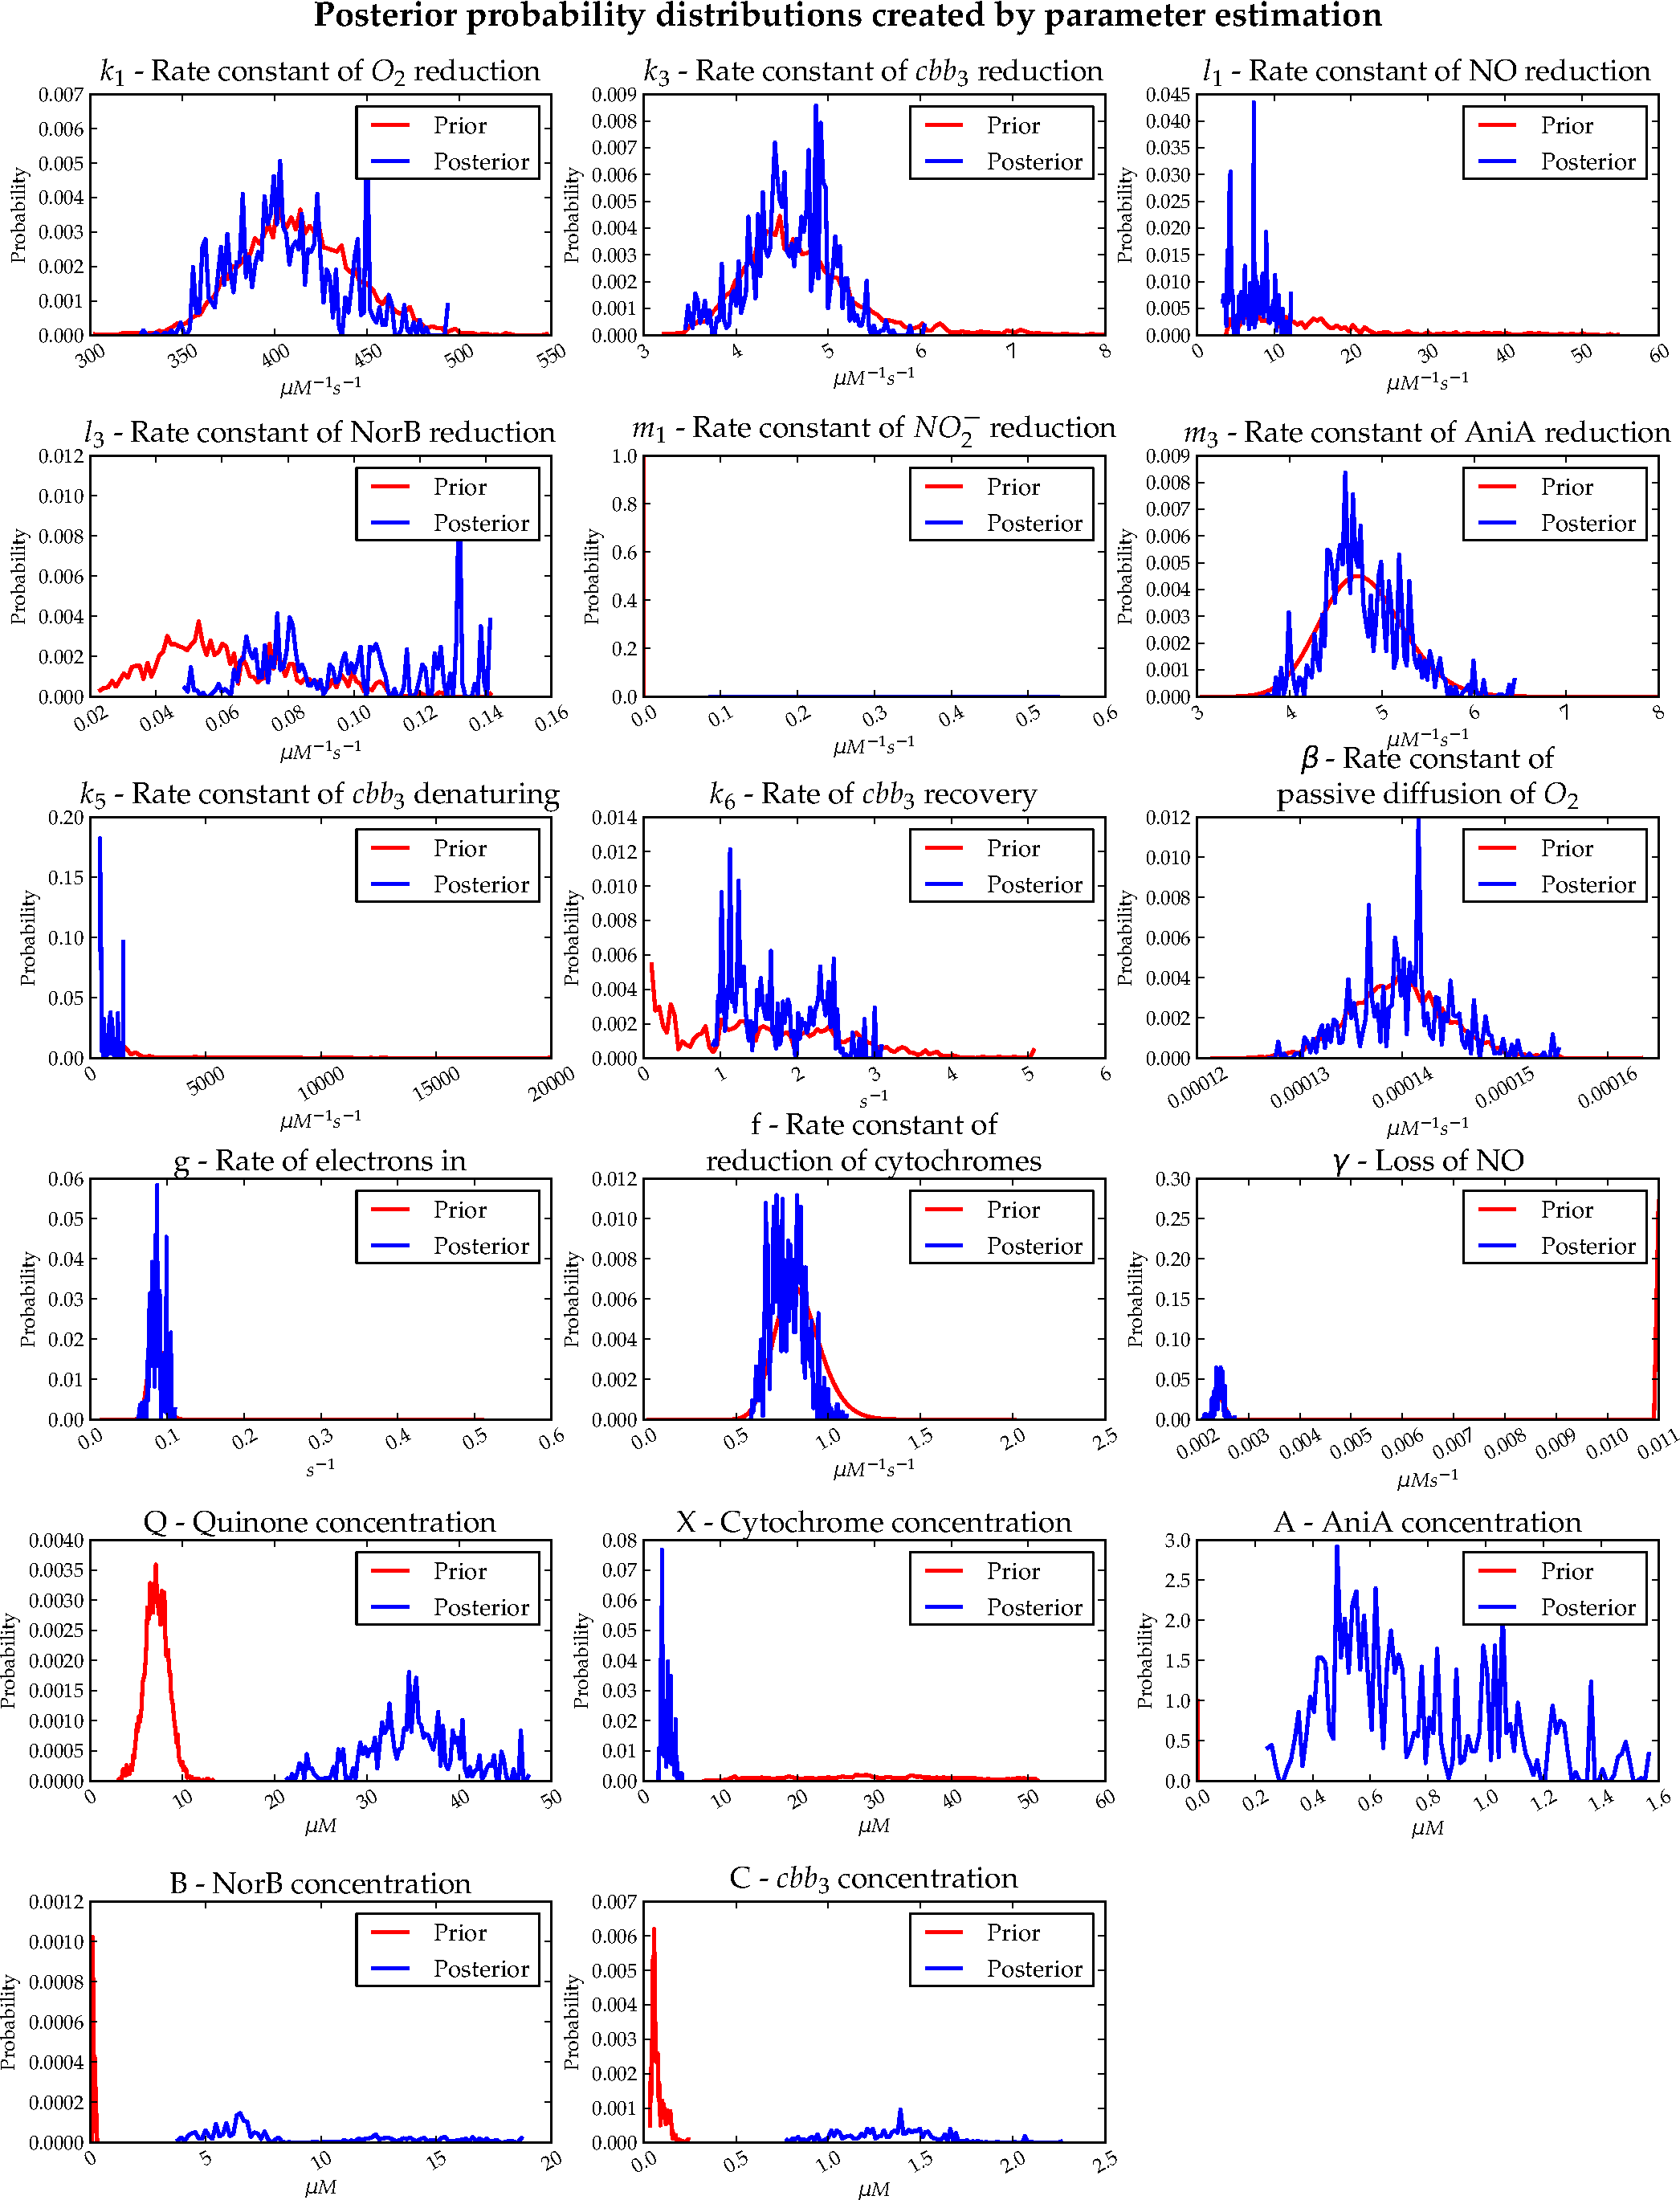
\includegraphics[width=15cm, trim=0cm 0cm 0cm 0cm, clip=true]{./07-nitritereduction/data/posteriors.pdf}
 % priors.pdf: 1008x1008 pixel, 72dpi, 35.56x35.56 cm, bb=0 0 1008 1008
 \caption[Posterior probability distributions for microaerobic oxygen and nitrite reduction]{{\bf Posterior probability distributions for microaerobic oxygen and nitrite reduction}. These are the final posterior probability distributions generated by the parameter estimation system for microaerobic oxygen and nitrite reduction, all concentrations have been normalised to assume an $OD_{600}$ of 1.
 \label{fig:nitrite_posteriors1}}
\end{figure}
\afterpage{\clearpage}

The idealised lognormal distribution parameters that fit the posterior probability distributions are shown in Table \ref{tab:nitrite-posteriors-table} and compared to the prior probability distributions.

\begin{table}[tbp]%needs to be 'here' as section is short
\renewcommand{\arraystretch}{1.5}
\begin{center}
\begin{tabular}{cccccc}
\toprule
& & \multicolumn{2}{c}{\textbf{Priors}} & \multicolumn{2}{c}{\textbf{Posteriors}} \\
\textbf{Parameter} && ${\bar{x}}$ & $\sigma$ & ${\bar{x}}$ & $\sigma$\\
\midrule
$k_1$ && 417.88 & 31.172 & 403.51 & 27.59\\
$k_3$ && 4.65 & 0.619 & 4.58 & 0.436\\
$l_1$ && 13.12 & 8.321 & 6.42$\downarrow$ & 2.33$\downarrow$\\
$l_3$ && 0.058 & 0.021 & 0.096 & 0.025\\
$m_1$ && 1 & 1 & 0.175$\downarrow$ & 0.087\\
$m_3$ && 4.8 & 0.2 & 4.79 & 0.042\\
$k_5$ && 1741.8 & 1822.0 & 138.66 ($\gamma = 399.86$)$\downarrow$ & 338.18$\downarrow$\\
$k_6$ && 1.076 & 1.473 & 1.59 & 0.527\\
$\beta$ && 0.00014 & $4.7\times 10^{-6}$ & 0.00014 & $4.7\times 10^{-6}$\\
g && 0.857 & 0.086 & 0.085$\downarrow$ & 0.0078$\downarrow$\\
f && 8.398 & 1.237 & 0.771$\downarrow$ & 0.096$\downarrow$\\
$\gamma$ && 0.0024 & $9\times 10^{-5}$ & 0.0024 & $8.8\times 10^{-5}$\\
Q && 7.06 & 1.317 & 34.31$\uparrow$ & 5.49$\uparrow$\\
X && 27.45 & 12.08 & 2.81$\downarrow$ & 0.595$\downarrow$\\
A && 0.137 & 0.048 & 0.704$\uparrow$ & 0.3$\uparrow$\\
B && 0.137 & 0.048 & 7.80$\uparrow$ & 3.63$\uparrow$\\
C && 0.071 & 0.029 & 1.3$\uparrow$ & 0.259$\uparrow$\\
\bottomrule
\end{tabular}
\end{center}
\caption[Posterior Probability Statistics]{{\bf Posterior Probability Statistics.} This table shows the parameters required to create lognormal distributions that describe the prior and posterior probability distributions. The values for the priors are as in Table \ref{tab:nitrite_prior_table}. The posterior distributions were generated from dataset 2, and where they relate to concentrations, these have been normalised. The lognormal distributions represent best-fits to the actual posterior distributions. Where there are significant differences between the prior and posterior values for either the mean or standard deviation, these are indicated by $\uparrow$ and $\downarrow$. Where a $\gamma$ value is shown in brackets it means that a 3 parameter lognormal had to be used, and $\gamma$ is the location parameter for the distribution.
\label{tab:nitrite-posteriors-table}}
\end{table}

As can be seen from Table \ref{tab:nitrite-posteriors-table} and Figure \ref{fig:nitrite_posteriors1} most of the rate constant probability distributions have remained fairly stationary throughout the multiple rounds of parameter estimation (from Chapters \ref{chap:oxygenreduction} \& \ref{chap:noreduction}). The distribution of $l_1$ has narrowed towards the lower and of the prior bounds. The distributions of $f$ and $g$ are almost identical to their modified prior distributions with very little deviation. The concentration distributions however have all been modified significantly from their prior distributions.

\subsection{Analysis of Convergence}
The Gelman-Rubin R statistics were calculated for the Monte-Carlo trajectories for each parameter and these are presented in Table \ref{tab:nitrite-r-stat}. These values show very high levels of convergence for all parameters, however it should be noted that these values may not be truly representative as in fact only 2 trajectories are being analysed here since these were the only ones that produced usable output.

\begin{table}[tbp]%needs to be 'here' as section is short
\renewcommand{\arraystretch}{1.5}
\begin{center}
\begin{tabular}{ccc|ccc}
\toprule
\textbf{Parameter} && \textbf{R Statistic} & \textbf{Parameter} && \textbf{R Statistic}\\
\midrule
$k_1$ && 1.07 & g && 1.03\\
$k_3$ && 1.06 & f && 2.27\\
$l_1$ && 1.30 & $\gamma$ && 1.02\\
$l_3$ && 2.89 & Q && 2.31\\
$m_1$ && 3.47 & X && 2.39\\
$m_3$ && 1.14 & A && 2.39\\
$k_5$ && 2.11 & B && 5.64\\
$k_6$ && 1.76 & C && 1.59\\
$\beta$ && 1.01\\
\bottomrule
\end{tabular}
\end{center}
\caption[Gelman-Rubin Convergence Statistic]{{\bf Gelman-Rubin Convergence Statistic.} This table shows the Gelman-Rubin Convergence statistic for the two Markov chains from dataset 2. For parameters which are concentrations, the statistic relates to the values after normalisation (data is normalised based on initial oxygen reduction rate).
\label{tab:nitrite-r-stat}}
\end{table}

\subsection{Analysis of Correlation}
Correlation analysis was performed on each of the parameters using the Monte-Carlo trajectories as in Chapters \ref{chap:oxygenreduction} and \ref{chap:noreduction}. The upper-triangle matrix in Figure \ref{tab:nitrite-regression}. There are quite a few cross correlations between parameters in this dataset, although they are all classed as ``moderate'' rather than ``high''. There are some obvious correlations such as the concentration of AniA and the reduction rate constant of Nitrite being negatively correlated, and that AniA and \cbbthree{} are negatively correlated to the concentration of cytochromes. This is explained by the fact that the more cytochromes, the faster AniA and \cbbthree{} can be reduced which means fewer are required to maintain the same level of substrate reduction. Interestingly \cbbthree{} and rate of reduction of oxygen do not appear to be correlated at all. This is most likely due to the fact that the reduction rate constant of oxygen by \cbbthree{} is so high that any oxygen is reduced almost instantaneously meaning that changes in that rate constant make very little difference if the concentration of \cbbthree{} is changed.

\begin{table}[p]
\setlength{\tabcolsep}{5pt}
\renewcommand{\arraystretch}{1.5}
  \centering
  \rotatebox{90}{
  \begin{minipage}{24.4cm}
  \centering
  \begin{tabular}{|c|c|c|c|c|c|c|c|c|c|c|c|c|c|c|c|c|c|c|}
    \hline
    \cellcolor{dark-gray} & \cellcolor{dark-gray}$k_1$ & \cellcolor{dark-gray}$k_3$ & \cellcolor{dark-gray}$l_1$ & \cellcolor{dark-gray}$l_3$ & \cellcolor{dark-gray}$m_1$ & \cellcolor{dark-gray}$m_3$ & \cellcolor{dark-gray}$k_5$ & \cellcolor{dark-gray}$k_6$ & \cellcolor{dark-gray}$\beta$ & \cellcolor{dark-gray}g & \cellcolor{dark-gray}f & \cellcolor{dark-gray}$\gamma$ & \cellcolor{dark-gray}Q & \cellcolor{dark-gray}X & \cellcolor{dark-gray}A & \cellcolor{dark-gray}B & \cellcolor{dark-gray}C\\ \hline
\cellcolor{dark-gray}$k_1$ & \cellcolor{light-gray}1 & 0.02 & 0.19 & 0.01 & -0.11 & 0.05 & 0.24 & -0.03 & 0.05 & -0.10 & -0.07 & 0.03 & 0.21 & -0.07 & 0.12 & 0.01 & -0.02\\ \hline
\cellcolor{dark-gray}$k_3$ & \cellcolor{light-gray} & \cellcolor{light-gray}1 & -0.03 & \cellcolor{orange}0.31 & \cellcolor{orange}-0.30 & -0.05 & 0.17 & -0.04 & 0.05 & 0.03 & -0.19 & -0.01 & 0.21 & \cellcolor{orange}-0.48 & \cellcolor{orange}0.44 & -0.14 & 0.25\\ \hline
\cellcolor{dark-gray}$l_1$ & \cellcolor{light-gray} & \cellcolor{light-gray} & \cellcolor{light-gray}1 & -0.21 & 0.15 & 0.22 & \cellcolor{orange}0.36 & -0.13 & -0.01 & -0.20 & -0.02 & 0.01 & 0.05 & \cellcolor{orange}0.43 & -0.07 & \cellcolor{orange}0.60 & \cellcolor{orange}-0.34\\ \hline
\cellcolor{dark-gray}$l_3$ & \cellcolor{light-gray} & \cellcolor{light-gray} & \cellcolor{light-gray} & \cellcolor{light-gray}1 & \cellcolor{orange}-0.52 & -0.25 & \cellcolor{orange}0.33 & -0.14 & 0.04 & 0.17 & \cellcolor{orange}-0.34 & -0.09 & \cellcolor{orange}0.36 & \cellcolor{orange}-0.49 & \cellcolor{orange}0.61 & \cellcolor{orange}-0.67 & \cellcolor{orange}0.46\\ \hline
\cellcolor{dark-gray}$m_1$ & \cellcolor{light-gray} & \cellcolor{light-gray} & \cellcolor{light-gray} & \cellcolor{light-gray} & \cellcolor{light-gray}1 & -0.10 & \cellcolor{orange}-0.53 & -0.12 & -0.02 & -0.04 & \cellcolor{orange}0.46 & 0.06 & \cellcolor{orange}-0.72 & \cellcolor{orange}0.64 & \cellcolor{orange}-0.75 & 0.26 & \cellcolor{orange}-0.52\\ \hline
\cellcolor{dark-gray}$m_3$ & \cellcolor{light-gray} & \cellcolor{light-gray} & \cellcolor{light-gray} & \cellcolor{light-gray} & \cellcolor{light-gray} & \cellcolor{light-gray}1 & 0.06 & 0.15 & 0.06 & 0.18 & 0.00 & 0.06 & 0.02 & -0.03 & -0.13 & \cellcolor{orange}0.34 & 0.02\\ \hline
\cellcolor{dark-gray}$k_5$ & \cellcolor{light-gray} & \cellcolor{light-gray} & \cellcolor{light-gray} & \cellcolor{light-gray} & \cellcolor{light-gray} & \cellcolor{light-gray} & \cellcolor{light-gray}1 & \cellcolor{orange}-0.46 & 0.03 & -0.13 & \cellcolor{orange}-0.41 & 0.02 & \cellcolor{orange}0.53 & \cellcolor{orange}-0.35 & \cellcolor{orange}0.60 & 0.01 & \cellcolor{orange}0.43\\ \hline
\cellcolor{dark-gray}$k_6$ & \cellcolor{light-gray} & \cellcolor{light-gray} & \cellcolor{light-gray} & \cellcolor{light-gray} & \cellcolor{light-gray} & \cellcolor{light-gray} & \cellcolor{light-gray} & \cellcolor{light-gray}1 & -0.09 & 0.17 & 0.22 & -0.03 & -0.11 & 0.00 & -0.09 & 0.09 & -0.04\\ \hline
\cellcolor{dark-gray}$\beta$ & \cellcolor{light-gray} & \cellcolor{light-gray} & \cellcolor{light-gray} & \cellcolor{light-gray} & \cellcolor{light-gray} & \cellcolor{light-gray} & \cellcolor{light-gray} & \cellcolor{light-gray} & \cellcolor{light-gray}1 & 0.13 & -0.01 & -0.03 & 0.05 & -0.07 & 0.06 & -0.06 & -0.03\\ \hline
\cellcolor{dark-gray}g & \cellcolor{light-gray} & \cellcolor{light-gray} & \cellcolor{light-gray} & \cellcolor{light-gray} & \cellcolor{light-gray} & \cellcolor{light-gray} & \cellcolor{light-gray} & \cellcolor{light-gray} & \cellcolor{light-gray} & \cellcolor{light-gray}1 & 0.06 & 0.0 & -0.19 & -0.25 & 0.17 & -0.25 & 0.12\\ \hline
\cellcolor{dark-gray}f & \cellcolor{light-gray} & \cellcolor{light-gray} & \cellcolor{light-gray} & \cellcolor{light-gray} & \cellcolor{light-gray} & \cellcolor{light-gray} & \cellcolor{light-gray} & \cellcolor{light-gray} & \cellcolor{light-gray} & \cellcolor{light-gray} & \cellcolor{light-gray}1 & 0.01 & \cellcolor{orange}-0.51 & 0.23 & \cellcolor{orange}-0.42 & 0.28 & -0.23\\ \hline
\cellcolor{dark-gray}$\gamma$ & \cellcolor{light-gray} & \cellcolor{light-gray} & \cellcolor{light-gray} & \cellcolor{light-gray} & \cellcolor{light-gray} & \cellcolor{light-gray} & \cellcolor{light-gray} & \cellcolor{light-gray} & \cellcolor{light-gray} & \cellcolor{light-gray} & \cellcolor{light-gray} & \cellcolor{light-gray}1 & -0.05 & 0.01 & -0.02 & 0.14 & 0.02\\ \hline
\cellcolor{dark-gray}Q & \cellcolor{light-gray} & \cellcolor{light-gray} & \cellcolor{light-gray} & \cellcolor{light-gray} & \cellcolor{light-gray} & \cellcolor{light-gray} & \cellcolor{light-gray} & \cellcolor{light-gray} & \cellcolor{light-gray} & \cellcolor{light-gray} & \cellcolor{light-gray} & \cellcolor{light-gray} & \cellcolor{light-gray}1 & \cellcolor{orange}-0.52 & \cellcolor{orange}0.78 & -0.16 & 0.24\\ \hline
\cellcolor{dark-gray}X & \cellcolor{light-gray} & \cellcolor{light-gray} & \cellcolor{light-gray} & \cellcolor{light-gray} & \cellcolor{light-gray} & \cellcolor{light-gray} & \cellcolor{light-gray} & \cellcolor{light-gray} & \cellcolor{light-gray} & \cellcolor{light-gray} & \cellcolor{light-gray} & \cellcolor{light-gray} & \cellcolor{light-gray} & \cellcolor{light-gray}1 & \cellcolor{orange}-0.74 & \cellcolor{orange}0.48 & \cellcolor{orange}-0.77\\ \hline
\cellcolor{dark-gray}A & \cellcolor{light-gray} & \cellcolor{light-gray} & \cellcolor{light-gray} & \cellcolor{light-gray} & \cellcolor{light-gray} & \cellcolor{light-gray} & \cellcolor{light-gray} & \cellcolor{light-gray} & \cellcolor{light-gray} & \cellcolor{light-gray} & \cellcolor{light-gray} & \cellcolor{light-gray} & \cellcolor{light-gray} & \cellcolor{light-gray} & \cellcolor{light-gray}1 & \cellcolor{orange}-0.33 & \cellcolor{orange}0.61\\ \hline
\cellcolor{dark-gray}B & \cellcolor{light-gray} & \cellcolor{light-gray} & \cellcolor{light-gray} & \cellcolor{light-gray} & \cellcolor{light-gray} & \cellcolor{light-gray} & \cellcolor{light-gray} & \cellcolor{light-gray} & \cellcolor{light-gray} & \cellcolor{light-gray} & \cellcolor{light-gray} & \cellcolor{light-gray} & \cellcolor{light-gray} & \cellcolor{light-gray} & \cellcolor{light-gray} & \cellcolor{light-gray}1 & \cellcolor{orange}-0.36\\ \hline
\cellcolor{dark-gray}C & \cellcolor{light-gray} & \cellcolor{light-gray} & \cellcolor{light-gray} & \cellcolor{light-gray} & \cellcolor{light-gray} & \cellcolor{light-gray} & \cellcolor{light-gray} & \cellcolor{light-gray} & \cellcolor{light-gray} & \cellcolor{light-gray} & \cellcolor{light-gray} & \cellcolor{light-gray} & \cellcolor{light-gray} & \cellcolor{light-gray} & \cellcolor{light-gray} & \cellcolor{light-gray} & \cellcolor{light-gray}1\\
\hline
  \end{tabular}
  \caption[Regression Analysis of Nitrite Reduction Parameters]{{\bf Regression Analysis of Nitrite Reduction Parameters for Dataset 2.} This table shows the $r$ values from linear regression analysis on the combined parameter trajectories for nitrite reduction. Parameters with high correlation have been coloured green ($R>0.8$) and those with moderation correlation have been coloured orange ($0.8>R>0.3$).
  \label{tab:nitrite-regression}}
  \end{minipage}
  }
\end{table}
\afterpage{\clearpage}

\subsection{Discussion}
The parameter estimates generated from this new set of data are capable of modelling experimental data particularly well, even if only in a qualitative manner. It also showed that the initial prior estimates for the values of $f$ and $g$ were (at least) an order of magnitude too high. These estimates were generated very early on in the modelling process during a trial-and-error period trying to find values that made sense biologically yet also allowed the model to fit the data. Impressively these initial values worked very well for most of the datasets where the nitrite pathway way note being employed, and it only became obvious in the later sets that these values were too high. The nitrite datasets showed that the rate of flow of electrons into the system was too high causing the cytochromes and quinone pool to stay in a permanently reduced state leading to very little change in enzyme activity when substrates were added or were depleted. The enzymes essentially had an unlimited supply of readily available electrons from both sources. Reducing the rate of both flow of electrons into the system, and the flow from the quinone pool to the cytochromes caused a massive change in the behaviour of the system as neither could be maintained in a fully reduced state. This completely altered the dynamics of the system as there was now true competition for electrons from the quinone pool and the cytochromes. The model became capable of modelling, in a qualitatively correct manner, the behaviour of the system when substrates were added and became depleted. Perhaps more impressively, none of the other rate constants needed to change, although the concentrations of the various enzymes were altered. Additionally the simple change of reducing the flux of electrons through the system actually brought the reduction states of the quinones and cytochromes into line with what was already published in the literature ($\approx$50\% reduced)\cite{Otten1999}.

\subsubsection[Using Nitrite Posterior Parameters]{Using Nitrite Posterior Parameters on Previous Datasets}
To further investigate the posteriors generated from parameter estimation, the best parameters that produced the output shown in Figure \ref{fig:nitrite_ds2_solved2} were used to create solved datasets for aerobic oxygen respiration, and for the addition of nitric oxide and compared against their equivalent experimental datasets. The enzyme concentrations were all scaled to match their respective datasets, and the solver was run using those parameters (no parameter estimation was performed). The results from these simulations are shown in Figures \ref{fig:oxygen_simulation}, \ref{fig:nitric_oxide_simulation} and \ref{fig:nitrite_simulation}.

\begin{figure}[tbp]
 \centering
 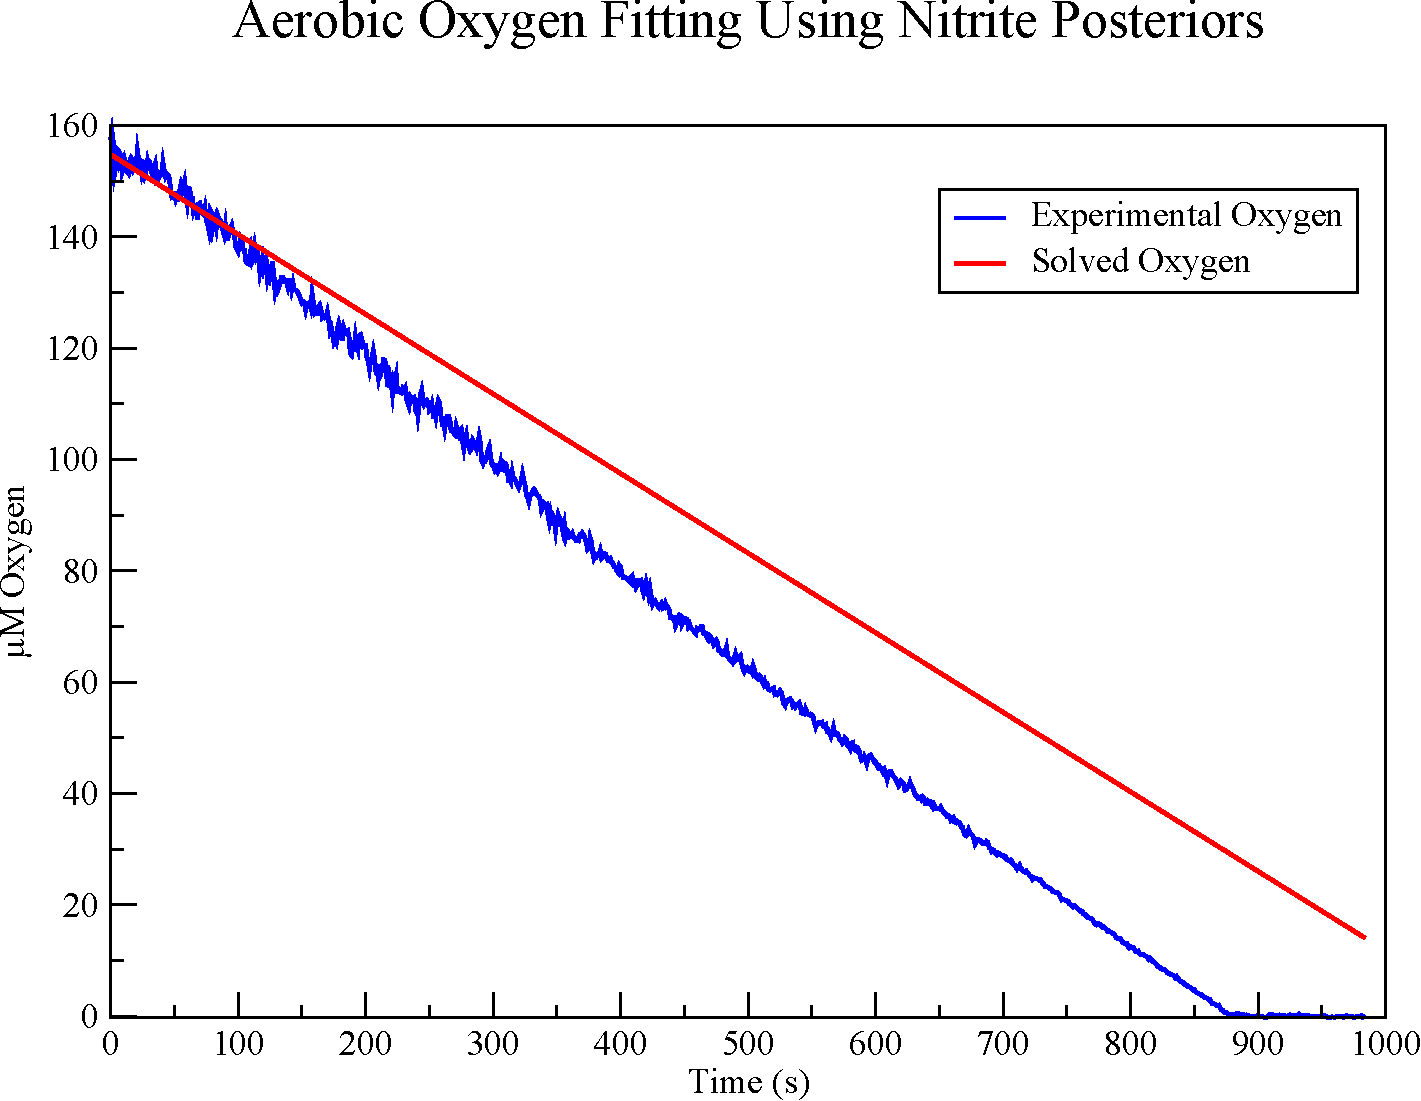
\includegraphics[height=10cm]{./07-nitritereduction/data/oxygen_dataset.pdf}
 % oxygen_dataset.pdf: 842x595 pixel, 72dpi, 29.70x20.99 cm, bb=0 0 842 595
 \caption[Aerobic Oxygen Respiration with Nitrite Posteriors]{{\bf Aerobic Oxygen Respiration with Nitrite Posteriors}. This figure shows the simulation results using the posteriors from nitrite parameter estimation with appropriately scaled concentrations.
 \label{fig:oxygen_simulation}}
\end{figure}

Figure \ref{fig:oxygen_simulation} shows the results of a simulation using the parameters obtained from nitrite parameter estimation compared to a simple aerobic oxygen reduction dataset. The concentration parameters have been appropriately scaled to match the experimental dataset (normalised based on observed oxygen reduction rate). The overall rate is too slow, however the simulation shows the same high affinity feature as the experimental dataset even with the reduced electron flux through the system. The difference in reduction rate is highly likely to be caused by the incomplete decoupling of cell culture density from other parameters.

\begin{figure}[tbp]
 \centering
 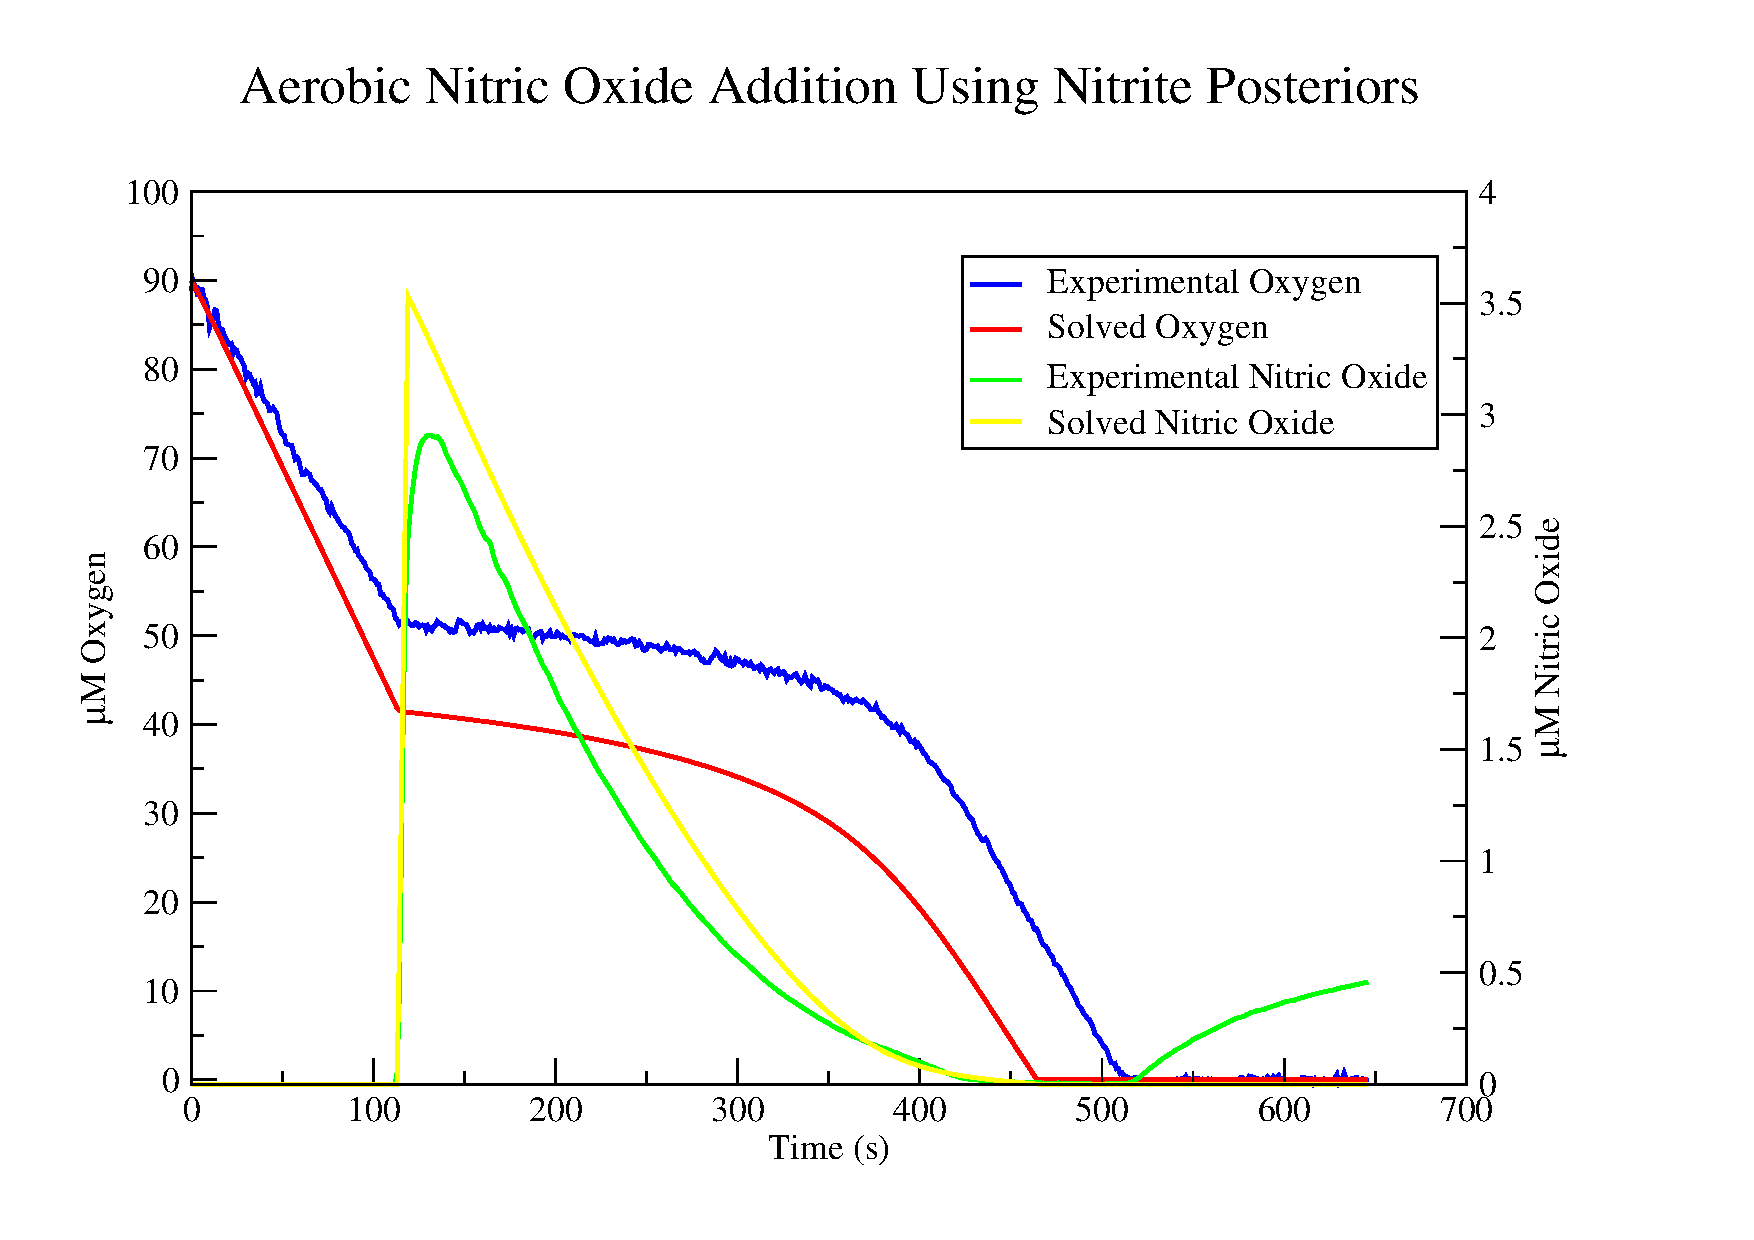
\includegraphics[height=10cm]{./07-nitritereduction/data/no_dataset.pdf}
 % no_dataset.pdf: 842x595 pixel, 72dpi, 29.70x20.99 cm, bb=0 0 842 595
 \caption[Aerobic Oxygen Respiration with Nitric Oxide Addition with Nitrite Posteriors]{{\bf Aerobic Oxygen Respiration with Nitric Oxide Addition with Nitrite Posteriors}. This figure shows the simulation results using the posteriors from nitrite parameter estimation with appropriately scaled concentrations. The concentration of NorB ($B$) had to be reduced significantly to obtained a similar nitric oxide reduction rate, and the value of $k_5$ had to be increased 66x to create a similarly shaped oxygen reduction curve.
 \label{fig:nitric_oxide_simulation}}
\end{figure}

Figure \ref{fig:nitric_oxide_simulation} shows the results of a simulation using the parameters obtained from nitrite parameter estimation compared to an aerobic oxygen reducing dataset where nitric oxide is added. The concentration parameters have been scaled appropriately to match the experimental dataset (as above). The concentration of NorB was altered further because this experimental dataset was not grown in microaerobic conditions and will not be expressing a high level of NorB. Thus NorB concentration was reduced to a value of $0.01~\mu M$. This was required to achieve a reasonable fit for the removal of nitric oxide. If the parameter obtained from nitrite fitting was used the nitric oxide was removed almost instantaneously. Additionally in order to produce a similarly shaped oxygen reduction curve, the value of $k_5$, the rate constant of \cbbthree{} inhibition by nitric oxide, had to be increased by $\approx 660\times$. This was required to reduce the rate of oxygen reduction to a suitable rate while there was nitric oxide present. The result is another qualitatively correct fit to the experimental data. The discrepancies again my be related to incorrect density decoupling.

\begin{figure}[tbp]
 \centering
 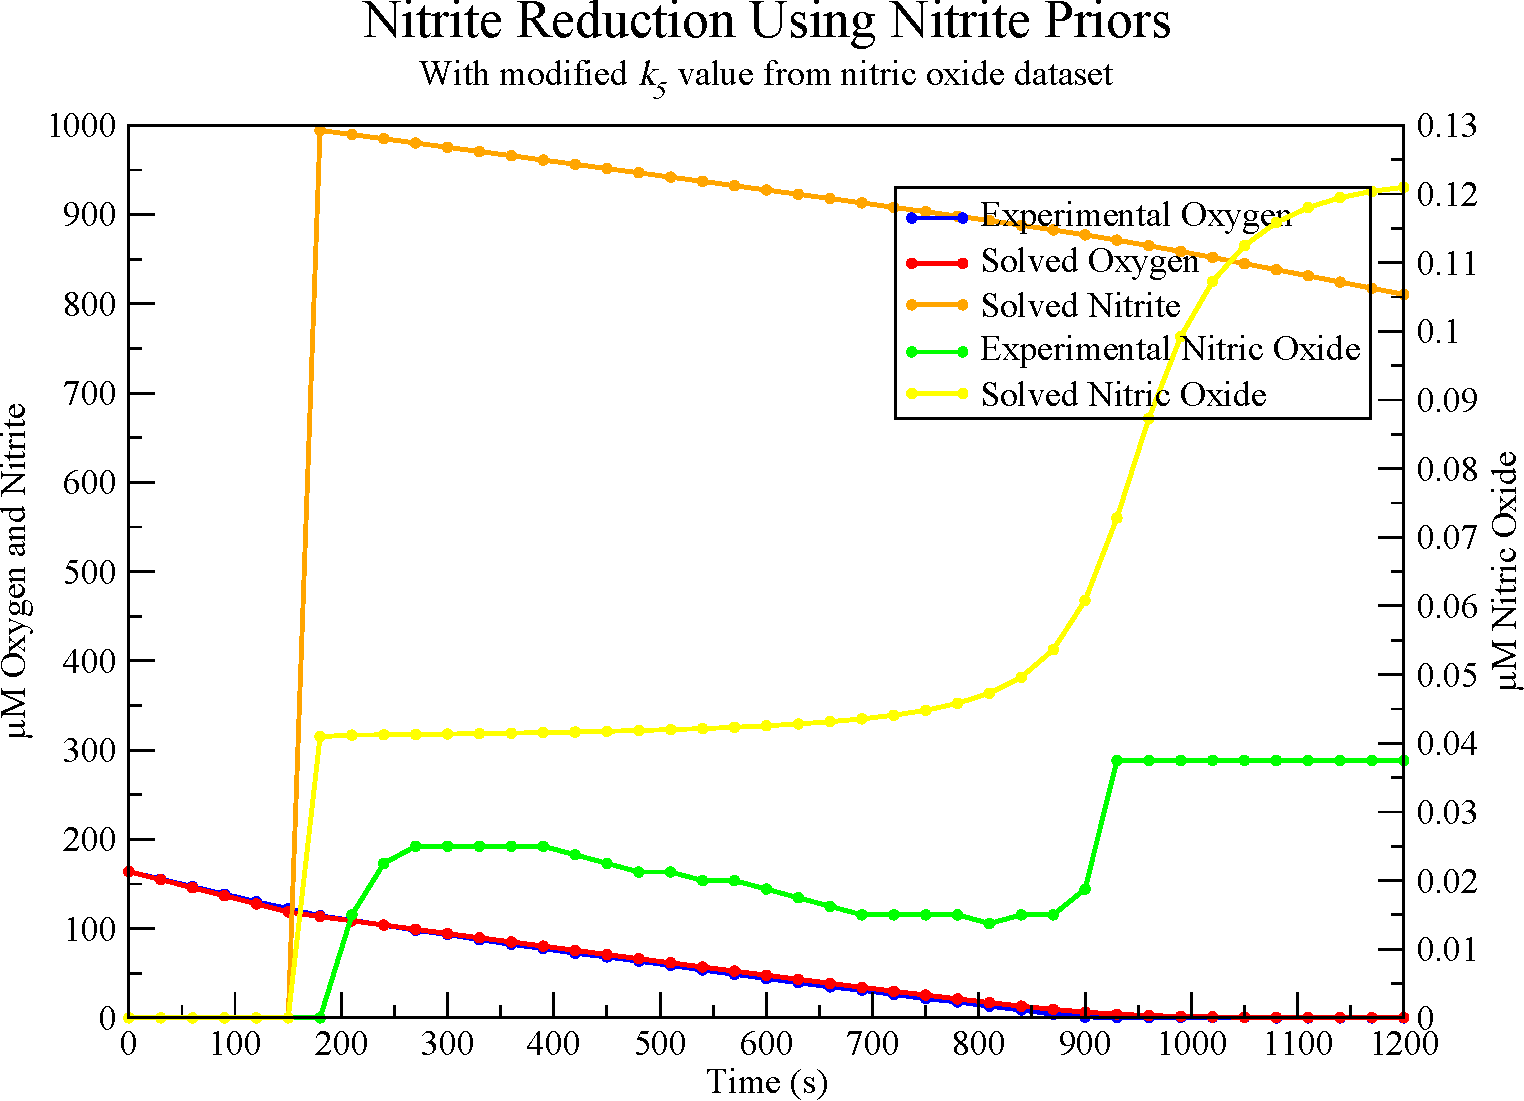
\includegraphics[height=10cm]{./07-nitritereduction/data/nitrite_dataset.pdf}
 % nitrite_dataset.pdf: 842x595 pixel, 72dpi, 29.70x20.99 cm, bb=0 0 842 595
 \caption[Nitrite Reduction using Modified Nitrite Posteriors]{{\bf Nitrite Reduction using Modified Nitrite Posteriors}. This figure shows the simulation results of the nitrite reduction dataset using the modified value of $k_5$ as described for Figure \ref{fig:nitric_oxide_simulation}. The change has not hugely affected the result except for making the increase in nitric oxide concentration when oxygen runs out a lot less sharp. This however may be closer to the \textit{in vivo} result. The experimental data is of a low enough resolution that it is very difficult to tell.
 \label{fig:nitrite_simulation}}
\end{figure}

Figure \ref{fig:nitrite_simulation} shows the results of a simulation using the nitrite posteriors with the same modification to $k_5$ as described for Figure \ref{fig:nitric_oxide_simulation}, to assess the difference it makes to the original result shown in Figure \ref{fig:nitrite_ds2_solved2}. The oxygen and nitrite results are almost identical, only the nitric oxide shows any significant change. The qualitative result is still very good as there is still an increase in nitric oxide concentration after oxygen runs out, however the change is much more sigmoidal that in the original simulation. This may not necessarily be a problem however as the original experimental data is of low resolution and would be incapable of capturing a more curved increase in nitric oxide concentration. It is highly likely in fact that both increases in nitric oxide concentration, after nitrite addition and after oxygen depletion are much more curved that the experimental data would suggest.

The fact that the value of $k_5$ can increase by such a large amount and only have such a limited effect on the outcome is due to the fact that the original parameter estimation results tended towards lower values where the probability was higher (as dictated by the priors). However increasing the value for $k_5$ would have had very little difference because the nitric oxide would be acting on vanishingly small concentrations of reduced \cbbthree{} since it spends most of its time in a fully oxidised state. In this case the posterior distribution is a little misleading as the value of this parameter actually has very little effect on the outcome of the simulation.